%% ---------------------------------------------
\RequirePackage{fix-cm}
%
%\documentclass{svjour3}                     % onecolumn (standard format)
%\documentclass[smallcondensed]{svjour3}     % onecolumn (ditto)
\documentclass[smallextended]{svjour3}   
\usepackage[english]{babel}
\usepackage{longtable}
\usepackage{graphicx}
\usepackage{amssymb}
\usepackage{amsmath}
\usepackage{color}
\usepackage{hyperref}
\usepackage{pifont}
%\usepackage{parskip}
\usepackage{fixltx2e}
\usepackage{array}
\usepackage[round]{natbib}
\bibliographystyle{plainnat}
\usepackage[normalem]{ulem}  
\usepackage{caption}
%\usepackage[T1]{fontenc}
\usepackage[utf8]{inputenc}
\usepackage{babel}
\usepackage[font=small,labelfont=bf]{caption}
\usepackage[switch]{lineno} 
\newcommand{\margin}[1]{\textcolor{red}{#1}} 
\newcommand{\out}[1]{\textcolor{green}{#1}} 
\usepackage{float} 
\usepackage{nomencl} 
\usepackage{ifthen} 
\renewcommand{\nomgroup}[1]{% 
  \ifthenelse{\equal{#1}{R}}{\item[\textbf{Roman Symbols}]}{%
    \ifthenelse{\equal{#1}{G}}{\item[\textbf{Greek Symbols}]}{%
      \ifthenelse{\equal{#1}{A}}{\item[\textbf{Abbreviations}]}{% 
        \ifthenelse{\equal{#1}{S}}{\item[\textbf{Subscripts}]}{% 
          \ifthenelse{\equal{#1}{U}}{\item[\textbf{Superscripts}]}{} 
        }% matches mathematical symbols
      }% matches Subscripts
    }% matches Abbreviations
  }% matches Greek Symbols
}% matches Roman Symbols
\renewcommand*{\nompreamble}{\footnotesize}
\usepackage{footnote} 
 \makenomenclature 
\renewcommand{\nomname}{Nomenclature}
\newcommand{\degree}{\ensuremath{^\circ}} 
\renewcommand{\arraystretch}{1.5}
\usepackage{framed} % Framing content
\usepackage{multicol} % Multiple columns environment
\renewcommand*\nompreamble{\begin{multicols}{2}}
\renewcommand*\nompostamble{\end{multicols}}
%\captionsetup[table]{skip=3pt}
\makeatletter
\newcommand*{\rom}[1]{\expandafter\@slowromancap\romannumeral #1@}
\makeatother
\newcommand{\nomunit}[1]{%
\renewcommand{\nomentryend}{\hspace*{\fill}#1}}
%\biboptions{square,compress}
\newcolumntype{P}[1]{>{\centering\arraybackslash}p{#1}}

%\usepackage[noheads,nomarkers]{endfloat}
\def\imagetop#1{\vtop{\null\hbox{#1}}}
\def\imagecenter#1{\raisebox{-0.5\height}{#1}}
\usepackage{amsfonts}
\newcommand{\overbar}[1]{\mkern 1.5mu\overline{\mkern-1.5mu#1\mkern-1.5mu}\mkern 1.5mu}
\usepackage[ampersand]{easylist}
\ListProperties(Hide=100, Hang=true, Progressive=3ex, Style*=-- ,
Style2*=$\bullet$ ,Style3*=$\circ$ ,Style4*=\tiny$\blacksquare$ )
\newcommand*\patchAmsMathEnvironmentForLineno[1]{%
\expandafter\let\csname old#1\expandafter\endcsname\csname #1\endcsname
\expandafter\let\csname oldend#1\expandafter\endcsname\csname end#1\endcsname
\renewenvironment{#1}%
{\linenomath\csname old#1\endcsname}%
{\csname oldend#1\endcsname\endlinenomath}}% 
\newcommand*\patchBothAmsMathEnvironmentsForLineno[1]{%
\patchAmsMathEnvironmentForLineno{#1}%
\patchAmsMathEnvironmentForLineno{#1*}}%
\AtBeginDocument{%
\patchBothAmsMathEnvironmentsForLineno{equation}%
\patchBothAmsMathEnvironmentsForLineno{align}%
\patchBothAmsMathEnvironmentsForLineno{flalign}%
\patchBothAmsMathEnvironmentsForLineno{alignat}%
\patchBothAmsMathEnvironmentsForLineno{gather}%
\patchBothAmsMathEnvironmentsForLineno{multline}%
}
\linenumbers
\usepackage[bottom]{footmisc}
\raggedbottom

\makeatletter
\def\@biblabel#1{}
\renewenvironment{thebibliography}[1]
     {\section*{\refname}%
      \@mkboth{\MakeUppercase\refname}{\MakeUppercase\refname}%
      \list{\@biblabel{\@arabic\c@enumiv}}%
           {\settowidth\labelwidth{\@biblabel#1{}}%
            \leftmargin\labelwidth
            \advance\leftmargin16pt
            \advance\leftmargin\labelsep
            \setlength\itemindent{-16pt}
            \@openbib@code
            \usecounter{enumiv}%
            \let\p@enumiv\@empty
            \renewcommand\theenumiv{\@arabic\c@enumiv}}%
      \sloppy
      \clubpenalty4000
      \@clubpenalty \clubpenalty
      \widowpenalty4000%
      \sfcode`\.\@m}
     {\def\@noitemerr
       {\@latex@warning{Empty `thebibliography' environment}}%
      \endlist}
%\renewcommand\newblock{\hskip .11em\@plus.33em\@minus.07em}
\makeatother

\makeatletter
\renewcommand{\@biblabel}[1]{{}\hfill}
\makeatother

\begin{document}

\title{Predicting Outdoor Thermal Comfort in Urban Environments: A New Numerical Model for Standard Effective Temperature}
\author{          Negin Nazarian \and
         Jipeng Fan \and 
         Tiffany Sin \and 
        Leslie Norford \and
        Jan Kleissl
}
\institute{N. Nazarian, Corresponding author \at
             1 University of California, San Diego, La Jolla, USA\\
             2 Singapore-MIT Alliance for Research and Technology, Singapore \\
             Tel.: +65 8285 4142, +1 858 699 9870\\
             \email{negin@smart.mit.edu}           %  \\
%             \emph{Present address:} of F. Author  %  if needed
\and
J. Fan, \at 
University of California, San Diego, La Jolla, USA
\and
           T. Sin \at
           Yale-NUS College, Singapore 
           \and 
           L. Norford \at
            Massachusets Institute of Technology, Cambridge, USA\and
           J. Kleissl \at
          University of California, San Diego, La Jolla, USA
}
\date{\today}

\maketitle
\begin{abstract}
With the rapid rate of urbanization, outdoor thermal comfort is becoming a growing health concern in densely-built areas. 
Therefore, in order to achieve comprehensive solutions to urban environmental problems, consideration of outdoor comfort alongside the building energy and urban wind flow analysis is crucial. In this study, outdoor thermal comfort, i.e. the human thermal sensation in response to the outdoor environment, is analyzed through a comprehensive index of Standard Effective Temperature (SET), and an improved methodology of predicting the spatial variability of thermal comfort is introduced. The improvement of the thermal comfort calculation is twofold. First, CFD simulations of the flow field coupled with the realistic urban surface heating are used to provide the input variables for the SET calculation. The CFD results provide detailed information on the unstable urban flow  as the most critical scenario to the human comfort. Second, the SET calculations are improved by introducing a detailed model of mean radiant temperature that incorporates  a) the visibility of urban surfaces to the pedestrians at any point, b) the spatial distribution of sky view factor, and c) inter-building  shadowing and shortwave radiation effects on thermal comfort. These improvements allow for evaluating the spatial distribution of SET at any level. Additionally, several sensitivity studies are  carried out for an idealized configuration representing a compact low rise urban zone. The SET evaluated at the pedestrian level (approximately 1.5-2 m from the ground) shows that urban density, wind patterns, and solar position concurrently influence thermal comfort. For example, a sensitivity study on the effect of urban density reveals that higher urban concentration can have favourable impact on the thermal comfort due to the increased shading, while the air temperature and consequently the energy demand are monotonically increased. The current study demonstrates the critical importance of a comprehensive thermal comfort model that considers the flow field patterns as well as the realistic heating distribution of surfaces, and describes a methodology to be expanded for more complex scenarios in order to further address the effect of urban design on thermal comfort and ultimately achieve people-centric design. 

\keywords{Computational Fluid Dynamics \and Mean Radiant Temperature \and Outdoor Thermal Comfort \and Standard Effective Temperature \and Urban Microclimate  }
\end{abstract}
%%%%%%%%%%%%%%%%%%%%%%%%%%%%%%%%%%%%%%%%%%%%%%%%%%%%%%%%%%%%%%%%%%%%%%%%%%%%%%%%%%%%%%%%%%%%%%%%%%%%%

\section{Introduction}
\label{intro}
In 2008, the global urban population exceeded the rural population for the first time in the history, and by 2050, two-thirds of the world population is expected to live in cities \citep{desa2014world}. While urbanization provides solutions for resource efficiency and financial growth, it also imposes a  variety of environmental challenges. One major environmental consequence of urbanization is the Urban Heat Island (UHI), i.e. the relative rise of temperature in densely built areas \citep{kim1992urban, oke1981canyon, oke1973city, bornstein1968observations}, which is responsible for significant economic and health concerns due to increased heat stress in densely built areas \citep{tan2010urban, lo2003land, mavrogianni2011comfort}. Consequently, the thermal sensation and experience of urban dwellers, i.e. thermal comfort, is shaped as a response to the UHI formation. 

Thermal comfort has been evaluated by means of measurements, surveys, and numerical methods; and thermal comfort indices that incorporate numerous microclimate factors have been introduced. Field studies \citep{chow_assessment_2016,lin_thermal_2009,nikolopoulou2001thermal} combined microclimate measurements and surveys from pedestrians in order to evaluate thermal comfort through both objective (microclimate) and subjective (physiological, psychological and behavioral) parameters. Such field studies have verified the role of urban design on the thermal sensation of urban dwellers, and are invaluable for understanding the complex nature of human comfort in urban area. However, field measurements fall short in 1) identifying and isolating the controllable variables in urban microclimates, and 2) representing the detailed spatial variability of thermal comfort indices. 

Numerical methods can further address these shortcomings. However, computing thermal comfort is complex in its nature, not only due to its subjectivity, but also due to the consideration of various parameters involved (such as air temperature, velocity, humidity, radiant temperature, and human metabolic rate). Accordingly, methods of describing thermal comfort, i.e. thermal comfort indices, vary in their assumptions and the thermal models that are based on \citep{gagge1971effective,azer1977,epstein2006thermal,honjo2009thermal}. For instance, the Predicted Mean Vote (PMV) was developed based on the Fanger comfort model \citep{fanger1967calculation, fanger1972thermal} as an empirically-based index, and is more applicable for field measurements of thermal comfort \citep{ye2003new}. Another commonly-used thermal comfort index is the Physiological Equivalent Temperature (PET), based on the Munich energy balance model for individuals (MEMI, \citet{honjo2009thermal}). In this study, Standard Effective Temperature (SET), which is an index developed from the Pierce two-nodes model \citep{oohori1984comparison}, is used to describe thermal comfort.  SET is a comprehensive metric that integrates the influences of air temperature, wind velocity, humidity,  radiation exposure and metabolic rate of humans on the thermal sensation. As it successfully relates all the environmental variables with a person’s thermal experience, it is one of the most commonly used thermal comfort indices \citep{ye2003new}. 

\begin{table*}[!t]
  \begin{framed}
  \footnotesize
    \printnomenclature
  \end{framed}
\end{table*}
Numerical modelling of outdoor thermal environment is a promising tool for evaluating the effect of design and various building technologies on the thermal comfort, but currently faces several challenges in computation.  Among the factors that add to the complexity of numerical thermal comfort analysis are a) the three-dimensional distribution of surface heating and temperature, and the consequent modification of the airflow and thermal fields; and b) the radiation exposure of pedestrians influenced by the urban forms and materials.  Complex urban geometry further exacerbates both of these challenges. The first category can be addressed by taking advantage of recent advancements in the CFD modeling of urban flow. One example of using detailed CFD simulations that consider the dynamic coupling of flow and thermal fields is discussed here. 

The second category draws attention to the importance of mean radiant temperature ($T_{mrt}$) representation, which accounts for pedestrian exposure to longwave and shortwave radiation. Due to the complexity of human radiant exposure, 
many thermal comfort models are limited in accuracy and in resolution of $T_{mrt}$ representation. For example, in the simulation done by Ali-Toudert and Mayer, $T_{mrt}$ is assumed to be equal to $T_{air}$ which is indeed far from the reality. Accordingly, several different methods for simulating $T_{mrt}$ in outdoor environments have been developed, including ENVI-met 3.1 \citep{bruse2004envi}, Rayman 1.2 \citep{matzarakis2007modelling}, CityComfort+ \citep{huang2014citycomfort+} and SOLWEIG 2.2 \citep{lindberg2008solweig}. However, these $T_{mrt}$ modelling methods have different limitations on accuracy or spatial prediction ability. ENVI-met is not user friendly, and requires users to manually transfer topography and vegetation pixels for each simulation. It is also computationally demanding and difficult to use on common desktop computers. Some studies have also questioned the validity of ENVI-met results in comparison to field measurements \citep{toudertdependence}. Rayman, on the other hand, is more user-friendly but can only simulate $T_{mrt}$ at one position per time \citep{huang2014citycomfort+}. Moreover, it does not account for reflected solar radiation, which results in low accuracy specifically for high albedo surfaces \citep{thorsson2007different}. SOLWEIG 2.2 has been shown to sacrifice accuracy due to a simplified radiation formula \citep{lindberg2008solweig}. CityComfort+ is still under development, and is limited in accuracy because it simplifies the calculation of longwave atmospheric radiation \citep{huang2014citycomfort+}.  Thus, in order to enhance the SET prediction in the outdoor environments, a more accurate model of $T_{mrt}$ in a three-dimensional geometry is needed.
\begin{figure}[t]
\graphicspath{ {image/} }
\centerline{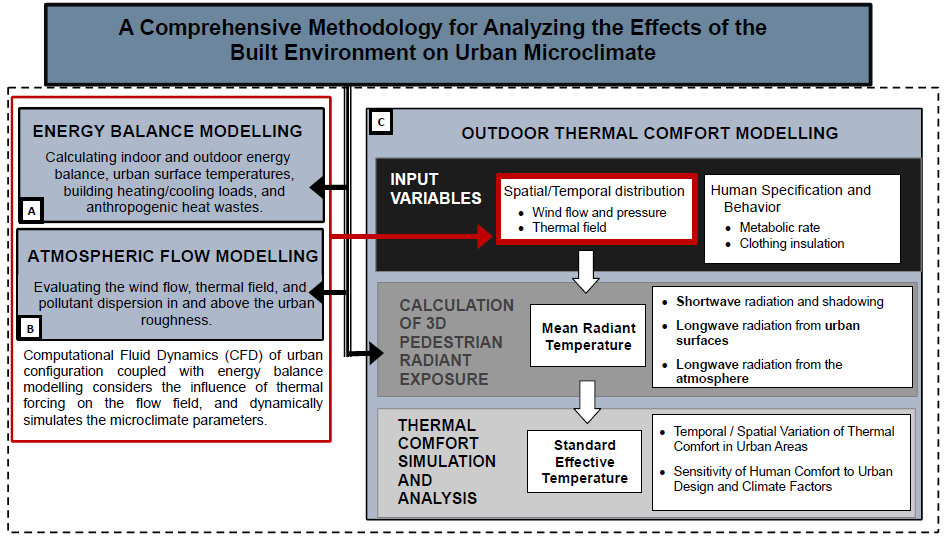
\includegraphics[width=\textwidth]{FlowChart_2.png}}
\caption{Flowchart of the research methodology for obtaining the detailed spatial distribution of thermal comfort.}
\label{Fig.FlowChart}
\end{figure}

The main objective of this study is to develop a comprehensive and accurate methodology of thermal comfort analysis, which can be further employed for evaluating the effect of urban design on humans' experiences.  Additionally, we aim to use this methodology for investigating the following questions: in urban configurations with realistic surface heating, what are the parameters that dominate the outdoor thermal comfort?  How does outdoor thermal comfort in urban areas varies in space; and do local or spatially-averaged values fully represent outdoor comfort? 
 
An overview of the research context and enhanced model set-up is shown in Figure \ref{Fig.FlowChart}. SET distributions are calculated using input parameters from the CFD simulation provided by \citet{nazarian2014effects, nazarian2015cfd} described in Sect. \ref{sec:cfd}. For calculating the thermal comfort index (SET in Sect. \ref{sec:set}), the CFD simulation is supplemented with an enhanced model of pedestrian radiant temperature (Sect. \ref{sec:mrt}). Additionally, the sensitivity of SET to several design and climate elements is evaluated for an idealized configuration of urban areas (Sect. \ref{sec:res}). Lastly, conclusions and future implications of this methodology are presented in Section \ref{sec:conc}. This paper completes the process of thermal comfort simulation from urban energy balance, air flow, and $T_{mrt}$ modeling to SET calculation. This method can be further developed and used to analyze thermal comfort in complex urban configurations.


%%%%%%%%%%%%%%%%%%%%%%%%%%%%%%%%%%%%%%%%%%%%%%%%%%%%%%%%%%%%%%%%%%%%%%%%%%%%%%%%%%%%%%%%%%%%%%%%%%%%%
%\nomenclature
\nomenclature[R]{$T$}{Temperature of each of corresponding mesh ($\rm K$)}%
\nomenclature[A]{$SET$}{Standard effective temperature ($\rm ^\circ C$)}%
\nomenclature[A]{$UHI$}{Urban Heat Island }%

\nomenclature[R]{$H_{sk}$}{Heat loss from the skin ($\rm W\, m^{-2}$)}%
\nomenclature[R]{$t_{so}$}{Standard operative temperature ($\rm K$)}%
\nomenclature[R]{$w$}{Skin wetness}%
\nomenclature[R]{$h_{es}$}{Standard evaporative heat transfer coefficient ($\rm W\, m^{-2}\,Pa^{-1}$)}%
\nomenclature[R]{$p_{ssk}$}{Water vapor pressure at skin temperature ($\rm kPa$)}%
\nomenclature[R]{$p_{SET}$}{Saturated water vapor pressure at standard effective temperature ($\rm kPa$)}%
\nomenclature[R]{$T_{mrt}$}{Mean radiant temperature ($\rm K$)}%
\nomenclature[G]{$\sigma$}{Stefan-Boltzmann constant ($\rm 5.67\times10^{-8}\, W m^{-2} K^{-4}$)}%
\nomenclature[G]{$a_{p}$}{Shortwave absorption coefficient of a person }%
\nomenclature[R]{$E_{sol}$}{Solar radiation intensity ($\rm W\, m^{-2}$)}%
\nomenclature[R]{$F_{sol-p}$}{View factor between the short-wave sources and a person}%
\nomenclature[G]{$\varepsilon_{sky}$}{Emissivity of the sky }%
\nomenclature[R]{$E_{sky}$}{Long-wave radiation intensity from the atmosphere ($\rm W\, m^{-2}$)}%
\nomenclature[R]{$F_{sky-p}$}{View factor between the visible sky and a person}%
\nomenclature[R]{$E_{urb}$}{Long-wave radiation intensity of urban surfaces ($\rm W\, m^{-2}$)}%
\nomenclature[G]{$\varepsilon_{urb}$}{Emissivity of urban surfaces  }%
\nomenclature[R]{$F_{urb-p}$}{View factor between urban surfaces and a person }%   
\nomenclature[R]{$P$}{Water vapor pressure ($\rm kPa$)}%
\nomenclature[R]{$h_{sp}$}{Standard heat transfer coefficient ($\rm W\, m^{-2}\,K^{-1}$)}%
%\nomenclature[R]{$SR$}{Total irradiance  ($\rm W\, m^{-2}$)}%
\nomenclature[R]{$v$}{Wind velocity  ($\rm m \, s^{-1})$}%

%%%%%%%%%%%%%%%%%%%%%%%%%%%%%%%%%%%%%%%%%%%%%%%%%%%%%%%%%%%%%%%%%%%%%%%%%%%%%%%%%%%%%%%%%%%%%%%%%%%%%

\section{Methods}
The solution strategy of the proposed work is discussed in the following sections. The calculation process is explained as a "grid-based" model (Sect. \ref{sec:gridModel})  that inputs the CFD results (Sect. \ref{sec:cfd})  for an idealized configuration representing compact mid-rise urban areas categorized by \citet{stewart2012local}. The basics of the standard effective temperature (SET) as a thermal comfort metric are then discussed in Section \ref{sec:set}, following a more detailed discussion on the mean radiant temperature calculation. 

It is also worth mentioning that SET simulation results in this study have been compared to the CBE Thermal Comfort Tool \cite{hoyt2013cbe} which is a licensed thermal comfort calculator for a given values of $T_mrt$, air temperature and speed. Furthermore, individual components of the simulation method have also been verified and validated. \citet{nazarian2014effects, nazarian2015cfd} validated the CFD results for air flow and surface temperature against various wind tunnel and airborne measurements. Additionally,  \cite{huang2014citycomfort+} verified the $T_{mrt}$ formula used in this paper (Eqn. \ref{Equ.MRT}), which is further improved by adding shade, sky view factor and urban surface visibility modeling. 
\subsection{Grid-Based Urban Model}
\label{sec:gridModel}
The geometry of the studied case consists of a 3x3 matrix of equally spaced cubic buildings (Fig. \ref{Fig.IdealUrban}). The framework of the SET calculation is defined by a mesh grid, wherein individual parameters are stored and analyzed along a grid reflecting the urban model. This allows for detailed analysis of spatial variation in thermal comfort and is further used to aid the calculation of $T_{mrt}$  explained in Sec. \ref{sec:visible}. SET values are calculated using MATLAB for a pedestrian standing at every point along the model.  

\begin {figure}[!h]
\graphicspath{ {image/} }
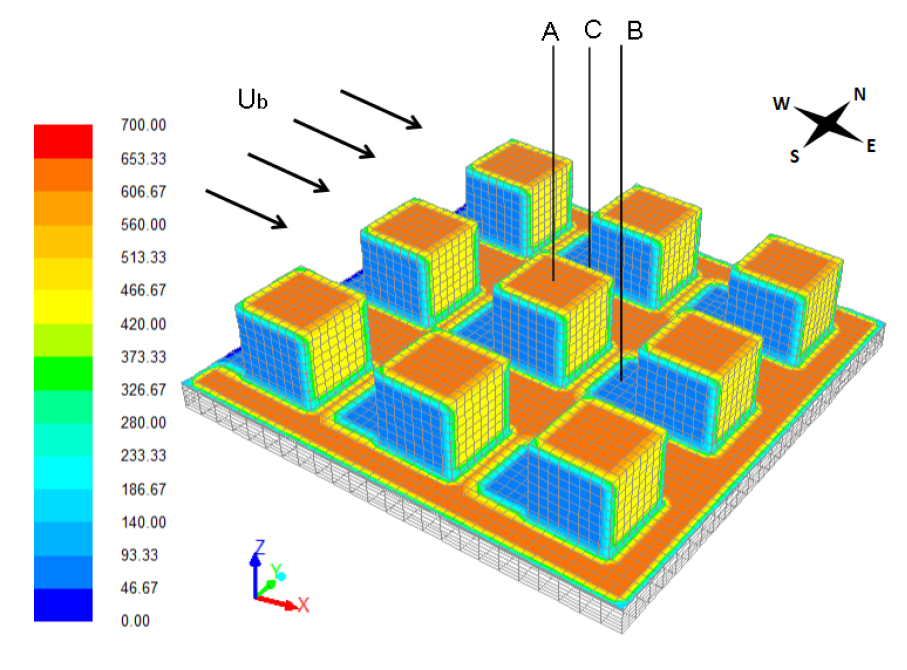
\includegraphics[width=7cm]{ThermalEnvironmentModel.PNG}
\centering
\caption{Idealized configuration of the urban environment used in CFD simulations by \citet{nazarian2014effects}}
\label{Fig.IdealUrban}
\end {figure}

%\begin{figure}[H]
%\graphicspath{ {image/} }
%\centering
%\subfigure[Cross-section of the urban model mesh]{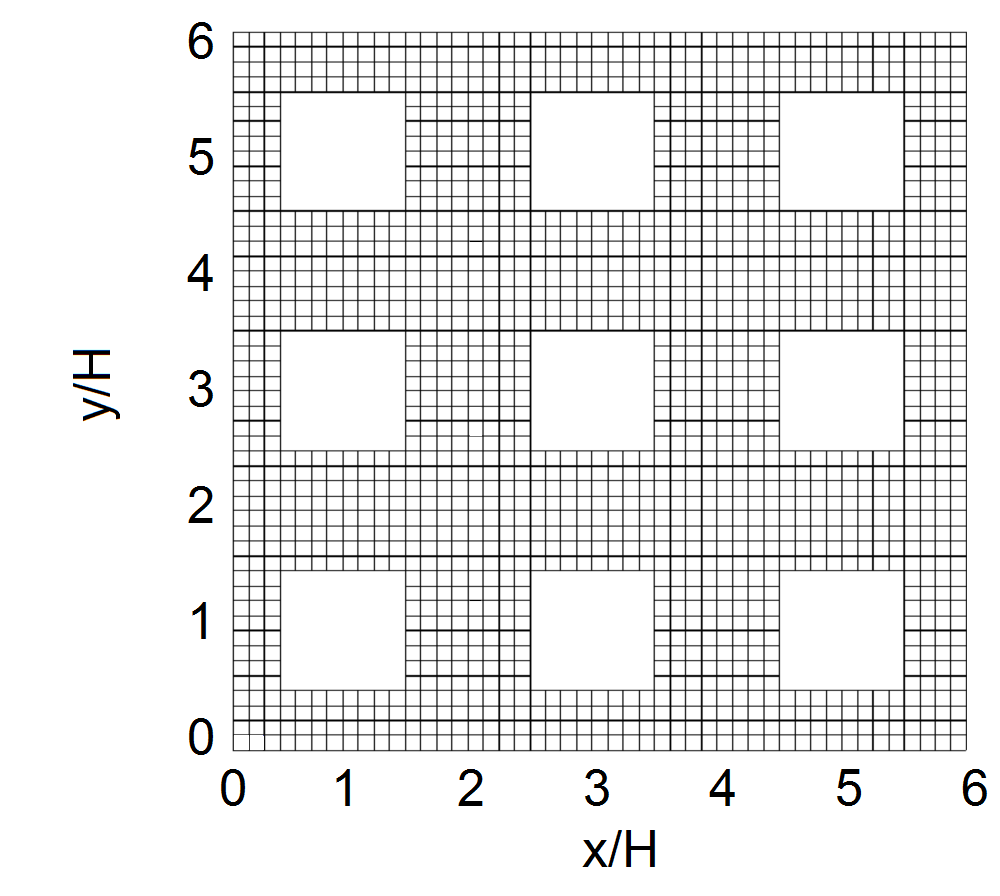
\includegraphics[width=2in]{groundold.png} }
%\hskip 0.4in 
%\centering
%\subfigure[Distribution of the air temperature at the pedestrian level (z=1.5 m) input from the CFD simulation at 1200 PST \cite{nazarian2014effects, nazarian2015cfd}]{
%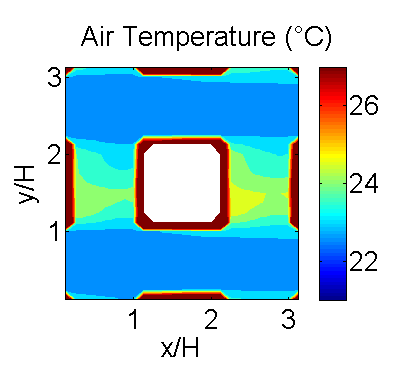
\includegraphics[width=2.2in]{AirTemp_BaseCase.png}}
%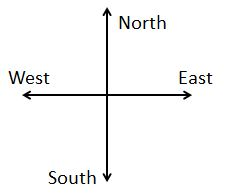
\includegraphics[width=1in]{ESWN.JPG}
%\caption{Parameters, such as temperature, are analyzed point by point throughout the mesh representing the urban model.}
%\label{Fig.GroundMesh}
%\end{figure}

\subsection{CFD Simulation Input}
\label{sec:cfd}
The 3D distribution of flow and thermal fields is taken from previous studies by  \citet{nazarian2014effects, nazarian2015cfd} that used a Computational Fluid Dynamic (CFD) model to simulate the urban microclimate for a 3D idealized configuration of a compact mid-rise urban environment (Fig. \ref{Fig.IdealUrban}). The simulations are done using the meteorological forcing data from a representative coastal urban weather station in southern California (San Diego, 32.867 N, 117.133 W) on a clear summer day, where the flow passes over a matrix of 3x3 evenly spaced buildings. Periodic boundary conditions are used such that the 3x3 configuration represents a unit cell within an array of infinite uniformly spaced buildings. Shortwave and longwave radiation are calculated at each time step and flow field is dynamically coupled with the thermal field. The model did not include windows on walls and latent heat flux is neglected. The simulation results were validated against field measurements and compared to other energy balance models. Refer to \cite{nazarian2014effects, nazarian2015cfd} for more information on the simulation setup and configuration.
%\vspace{3ex}

\subsection{Calculation of Standard Effective Temperature}
\label{sec:set}
While the CFD simulations provide detailed information on the climate characteristics, they are not sufficient for understanding thermal comfort. Human sensation of the thermal environment is affected by the combined and counteracting effects of several parameters, including wind, temperature, and radiant heat transfer from the human body, that are not fully represented in the CFD results. 

Accordingly, standard effective temperature (SET) is the index chosen to quantify and fully analyze thermal comfort. The standard effective temperature (SET) is defined as the equivalent temperature of an isothermal environment at 50 percent relative humidity at which a subject, while wearing typical clothing, would have the same heat stress (skin temperature, $T_sk$ ) and thermoregulatory strain (skin wetness, w) as in the actual test environment. Based on the dynamic Pierce two-node model of human temperature regulation, SET accounts for both body skin and body core. The body core node represents the metabolic system and heat exchange inside the body, and the body skin node represents skin, perspiration system, clothes and external heat exchange. The equation for SET is  expressed by \cite{gagge1986standard} as\\
\begin{equation}
H_{sk}=h_{sp}(t_{so}-SET)+wh_{es}(P_{ssk}-0.5P_{SET})
\label{Eqa.SET}
\end{equation}\\
where $H_{sk}$ ($\rm W\, m^{-2}$) is the heat loss from skin; $h_{sp}$ ($\rm W\, m^{-2}\,K^{-1}$) is the standard heat transfer coefficient; $t_{so}$ ($K$) is the standard operative temperature; $w$ (-) is the fraction of the wetted skin surface; $h_{es}$ ($\rm W\, m^{-2}\,Pa^{-1}$) is the standard evaporative heat transfer coefficient; $P_{ssk}$ ($\rm kPa$) is the water vapor pressure at skin, assumed to be that of saturated water vapor at skin temperature; and $P_{SET}$ ($\rm kPa$) is the saturated water vapor pressure at SET. In this study, SET ($^{\circ}$C) is analyzed as a steady state without significant heat storage within the body. Therefore, $H_{sk}$ is assumed to be zero. The accuracy of SET calculations are improved by modelling mean radiant temperature (Sect. \ref{sec:mrt}), which contributes to $t_{so}$, the standard operative temperature. 


\subsection{Mean Radiant Temperature Modeling}
\label{sec:mrt}
The effect of radiation on the thermal sensation is represented by mean radiation temperature ($T_{mrt}$), which is the uniform temperature of an imaginary enclosure in which radiant heat transfer from the human body is equal to those in the actual non-uniform enclosure. $T_{mrt}$ is a key factor in calculating the standard operating temperature ($t_{so}$) and thus is an important variable in human thermal comfort. Outdoor simulations of $T_{mrt}$ are difficult due to the urban complex geometry and the transient inter-building shadowing and radiation balance. 

In this study, the $T_{mrt}$ calculations are built upon the method introduced by \citet{huang2014citycomfort+} for simulating the spatial variation of $T_{mrt}$.  \citet{huang2014citycomfort+} derives $T_{mrt}$ by modeling three primary components of radiation fluxes: shortwave radiation (diffuse, direct and reflected), atmospheric longwave radiation from the sky, and longwave radiation from urban surfaces. Each component is weighted by their view factors relative to the position of the pedestrian:\\
\begin{equation}
T_{mrt}=\sqrt[4]{\frac{1}{\sigma}(a_{p}{\cdot}E_{sol}{\cdot}F_{sol\rightarrow{p}}+\varepsilon_{sky}{\cdot}E_{sky}{\cdot}F_{sky\rightarrow{p}}+\varepsilon{\cdot}E_{urb}{\cdot}F_{urb\rightarrow{p}})}
\label{Equ.MRT}
\end{equation}

The first term in Eq. \ref{Equ.MRT} denotes the shortwave radiation from sun, i.e. direct solar radiation. The second term is the atmospheric longwave radiation, and the third term is the longwave radiation from urban surfaces. The accuracy of this method is verified by \citet{huang2014citycomfort+}. However, in order to simplify the simulation, shading effects are ignored and the sky view factor, $F_{sky\rightarrow{p}}$, is assumed to be constant. Thus, to further improve spatial accuracy of $T_{mrt}$ and consequently SET calculation, this study further enhances the model by including the variation of shade and sky view factor within the building area.

\subsubsection{Shortwave radiation and shade modeling}
Shortwave radiation denotes the sum of the intensity of direct solar radiation, diffuse solar radiation and reflected radiation. To simulate solar radiation in the idealized urban area of this study, the solar ray-tracing algorithm of ANSYS FLUENT 14.5 is adopted to calculate the sun position and direct normal irradiance (DNI). Additionally, since diffuse radiation is considered to be uniform in numerical simulations \cite{flint1998solar, sreekumar1998egret, madronich1999role}, and reflected radiation is only a small proportion of the total radiation (Fig. \ref{Fig.SolarIntensity}), this paper considers both diffuse and reflected radiation as isotropic. However, as the direct solar radiation is the most dominant component, the sunlit areas are distinguished from the shade by using a vector-geometry shading algorithm that determines if the solar ray intersect with the the candidate grid. Equation \ref{Equ.Shad} explains the geometrical relations for determining the shade location according to solar position, and the schematic of the shading model is further demonstrated in Fig. \ref{Fig.Shadow}. 

\begin{figure}[!h]
\graphicspath{ {image/} }
\centerline{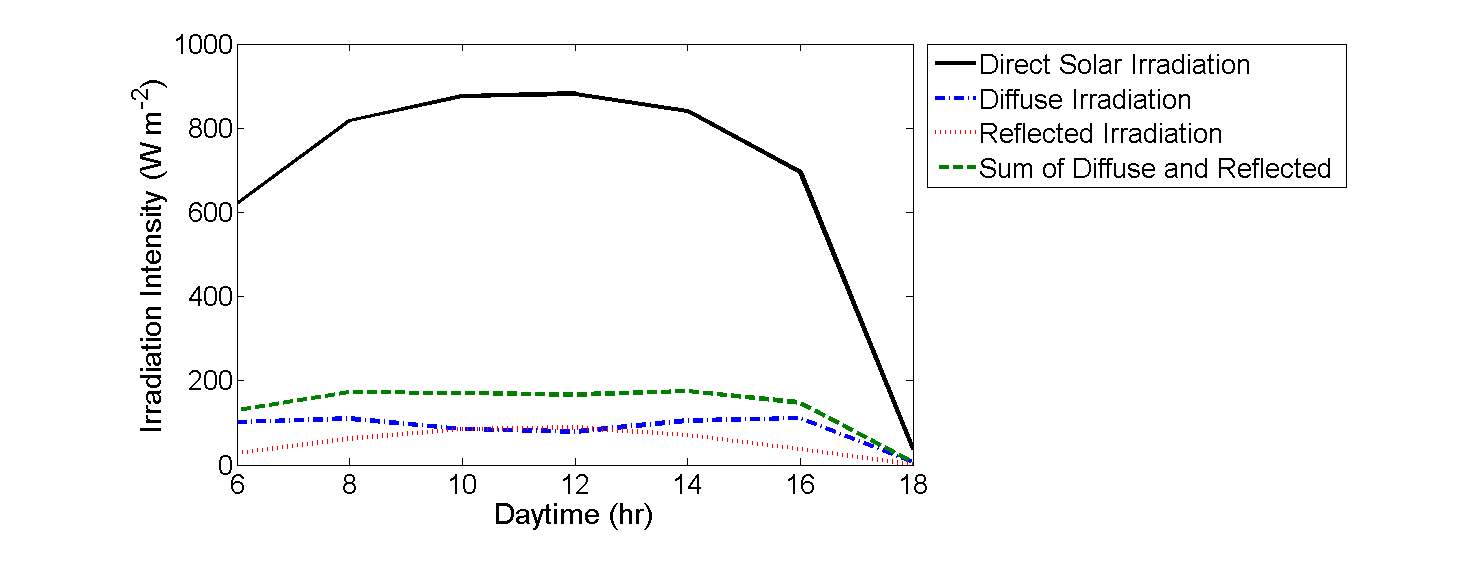
\includegraphics[width=14cm]{solar_intensity.png}}
\caption{Decomposition of daily solar radiation at the pedestrian level.}
\label{Fig.SolarIntensity}
\end{figure}

\begin{figure}[!h]
\graphicspath{ {image/} }
\centerline{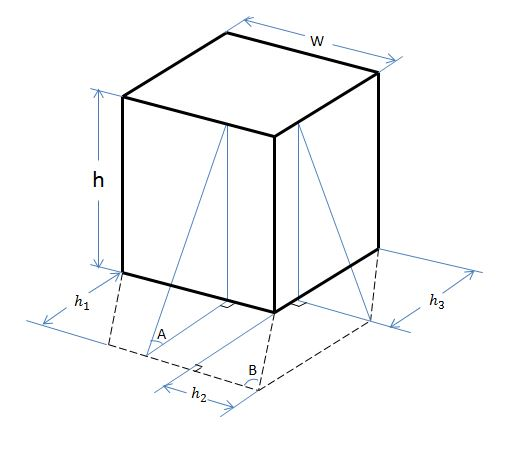
\includegraphics[width=0.6\textwidth]{SVFModel.JPG}}
\caption{The schematic of the shadow model  where the dashed lines indicate edges of shaded area.}
\label{Fig.Shadow}
\end{figure}


\begin{equation}
\centering
\begin{split}
A=&atan(\frac{x}{y})\\
h_1=&\frac{h}{tan(A)}\\
B=&atan(\frac{y}{z})\\
h_2=&\frac{H_1}{tan(B)}\\
h_3=&\frac{H_2}{tan(90-B)}
\end{split}
\label{Equ.Shad}
\end{equation}
In Eq. \ref{Equ.Shad}, x,y,z are solar beam vector components from the ray-tracing algorithm. These geometric calculations of shading effects substantially enhance the accuracy of direct solar radiation, and consequently thermal comfort calculations. For example, Fig. \ref{Fig.ShadowExample} shows the results derived from the shade model for the urban configuration at 1000 PST. It can be seen that the shade is present at the west side of the buildings while also covering a smaller area to the north of the building. As a pedestrian standing in a street canyon, with the same value of air temperature and wind velocity, the thermal sensation would be significantly different based on the position of the shaded areas, which further emphasize on the importance of including such shade model for the thermal comfort calculation. 

\begin{figure}[!h]
\graphicspath{ {image/} }
\begin{tabular}{cc}
   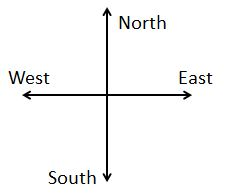
\includegraphics[width=1in]{ESWN.JPG} & 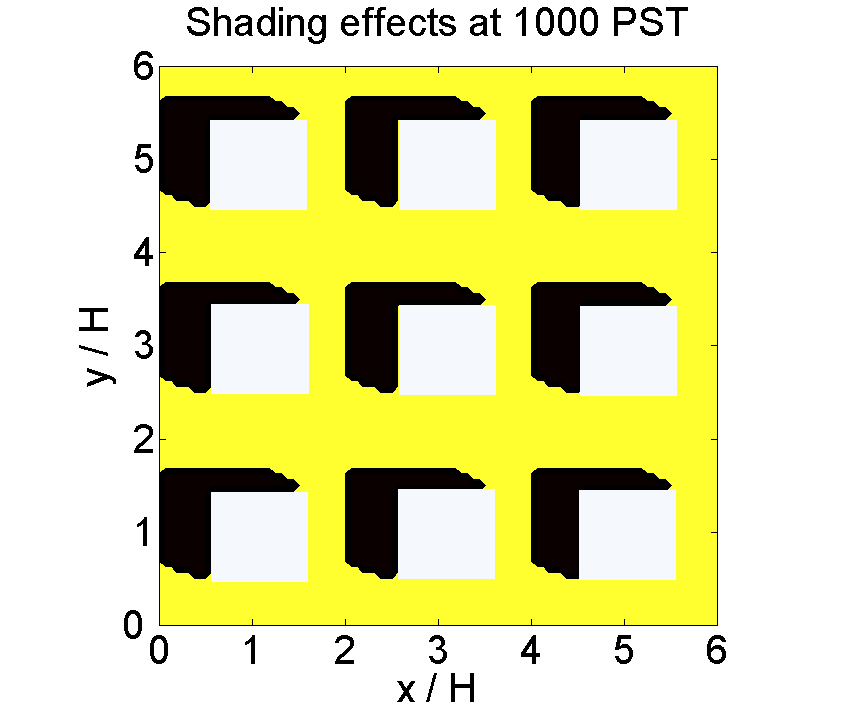
\includegraphics[width=0.5\textwidth]{ShadowSample.png}  
\end{tabular}
\caption{An example of shade configuration calculated at 1000 PST. Black regions indicate shaded area; while yellow is sunlit.}
\label{Fig.ShadowExample}
\end{figure}

\subsubsection{Longwave radiation from the atmosphere and sky view factor modeling}
In addition to shortwave radiation, mean radiant temperature also depends on sky longwave radiation, which describes the radiation emitted from atmosphere. To improve the accuracy of Huang's $T_{mrt}$ model, longwave radiation from the sky needs to be weighted by the sky view factor (SVF). SVF is calculated as the fraction of sky visible when viewed from the ground up.  \cite{wu2013calculation} introduces a simplified estimation method of SVF in urban areas without sacrificing spatial accuracy. Wu’s method begins with calculating the wall view factor (WVF) using the azimuths ($\gamma$) and altitude ($\beta$) angles to the building.\\
\begin{equation}
\rm
WVF_{M2}=\frac{1}{2\pi}
\left\{
(\gamma_2-\gamma_1)+cos{\beta}[tan^{-1}(cos{\beta}tan{\gamma_1})-tan^{-1}(cos{\beta}tan\gamma_2)]
\right\}
\end{equation}\\
\begin{equation}
SVF_{ref-M2}=1-(WVF_{1-M1}+WVF_{2-M2})
\end{equation}\\
where $WVF_{M1}$ and $WVF_{M2}$ indicate wall view factor in two different directions. An example of SVF modeling that is used in this study is presented in Figure \ref{Fig.SVFexample}, where the canyon aspect ratio is 1:2. 

\begin{figure}[!h]
\graphicspath{ {image/} }
\centerline{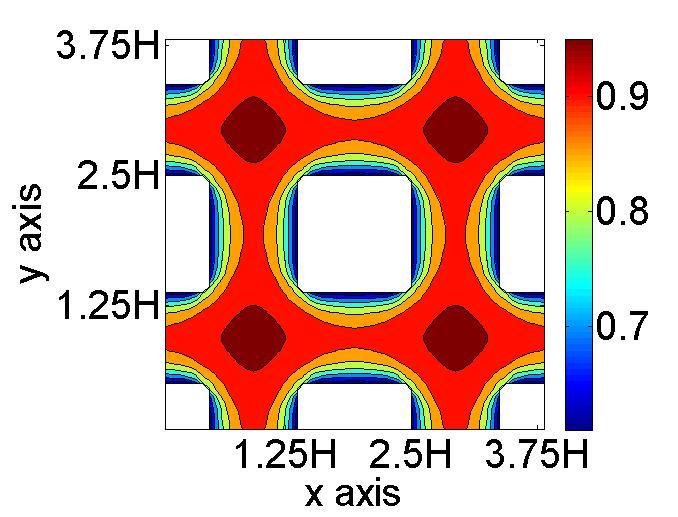
\includegraphics[width=0.6\textwidth]{SVFSample.jpg}}
\caption{The spatial distribution of sky view factor modelled around one building with canyon aspect ratio 0.5.}
\label{Fig.SVFexample}
\end{figure}
\subsubsection{Longwave radiation from urban surfaces and urban surface visibility modeling}
\label{sec:visible}
The third term of $T_{mrt}$ in Eq. \ref{Equ.MRT} describes longwave radiation  released from building and ground surfaces. Only visible surfaces can generate longwave radiation that affects the pedestrian's thermal sensation. To model this component of $T_{mrt}$, the temperature of each surface must be weighted by view factors, i.e. the proportion of radiation released from surface A that strikes surface B. The grid-based model explained in \ref{sec:gridModel} is used to calculate the view factor between two different points with a simple algorithm.

The algorithm analyzes a line between two different urban ground surfaces and checks if the line intersects with any buildings (i.e. whether the radiation between these two points are blocked). A visibility matrix is then generated and stored at each pedestrian location. This is done in three dimensions based on a point at pedestrian height using the grid-based model. 

Figure \ref{Fig.VisibilityExample} show examples of visibility modeling at pedestrian height, each with respect to analysing point, i.e. pedestrian position, at (1.875H, 1.875H) and (1.875H, 3.125H).
\begin{figure}[H]
\centering  
\graphicspath{ {image/} }
\begin{tabular}{cc}
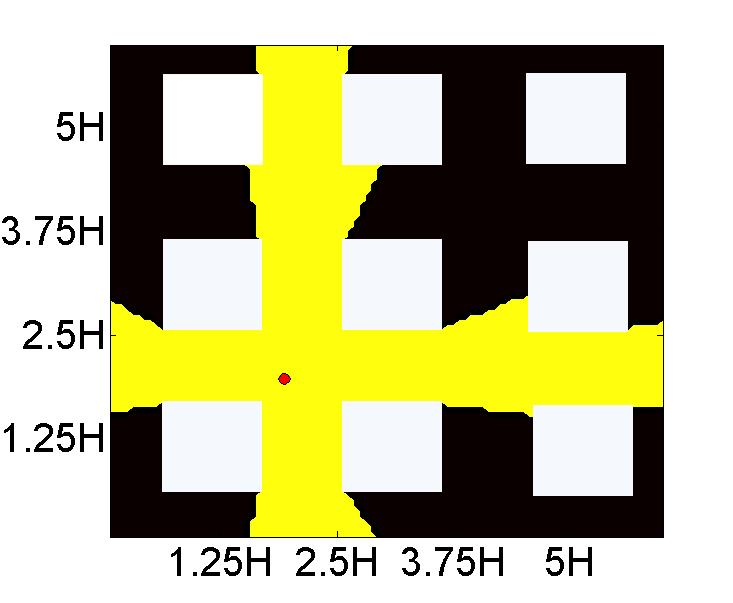
\includegraphics[width=0.4\textwidth]{VisibilityTestExampleOne.jpg}   &
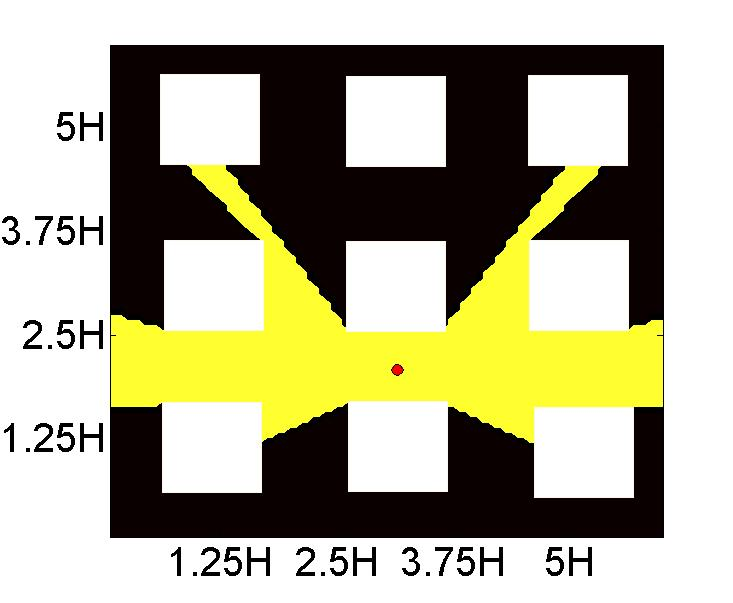
\includegraphics[width=0.4\textwidth]{VisibilityTestExampleTwo.jpg}
\end{tabular}
\caption{Examples of visibility modelling where the red dot denotes object standing position; yellow indicate visible area; black is the invisible area;  and white denotes building projection. }
\label{Fig.VisibilityExample}
\end{figure}



%%%%%%%%%%%%%%%%%%%%%%%%%%%%%%%%%%%%%%%%%%%%%%%%%%%%%%%%%%%%%%%%%%%%%%%%%%%%%%%%%%%%%%%%%%%%%%%%%%%%%
\section{Simulation Results}
\label{sec:res} 
The following section describes the calculation results of thermal comfort in urban area, which are simulated with the following assumptions: The testing subject is a man with typical summer clothes weighing 70 kg and 173 cm tall, standing  in the urban area of San Diego, California in a clear summer day. The calculations are made at the pedestrian level of 1.5 meters from ground. Average wind velocity is 2 m/s at the forcing height of 2H, where H is the building height. 


\subsection{Spatial variation of thermal comfort}
Thermal comfort values are represented as SET distributions in a horizontal cross-section at the pedestrian height. In order to identify the dominant factors in thermal comfort, the SET distribution in Fig. \ref{Fig.Parameters} is compared to the initial inputs from the CFD results such as air temperature, wind velocity, and ground temperature at 1000 PST (Fig. \ref{Fig.Parameters}). Several other parameters, such as sky view factor and pressure, are not shown explicitly but incorporated into the $T_{mrt}$ calculation.  

\begin{figure}[!h] \centering  
\graphicspath{ {image/} }
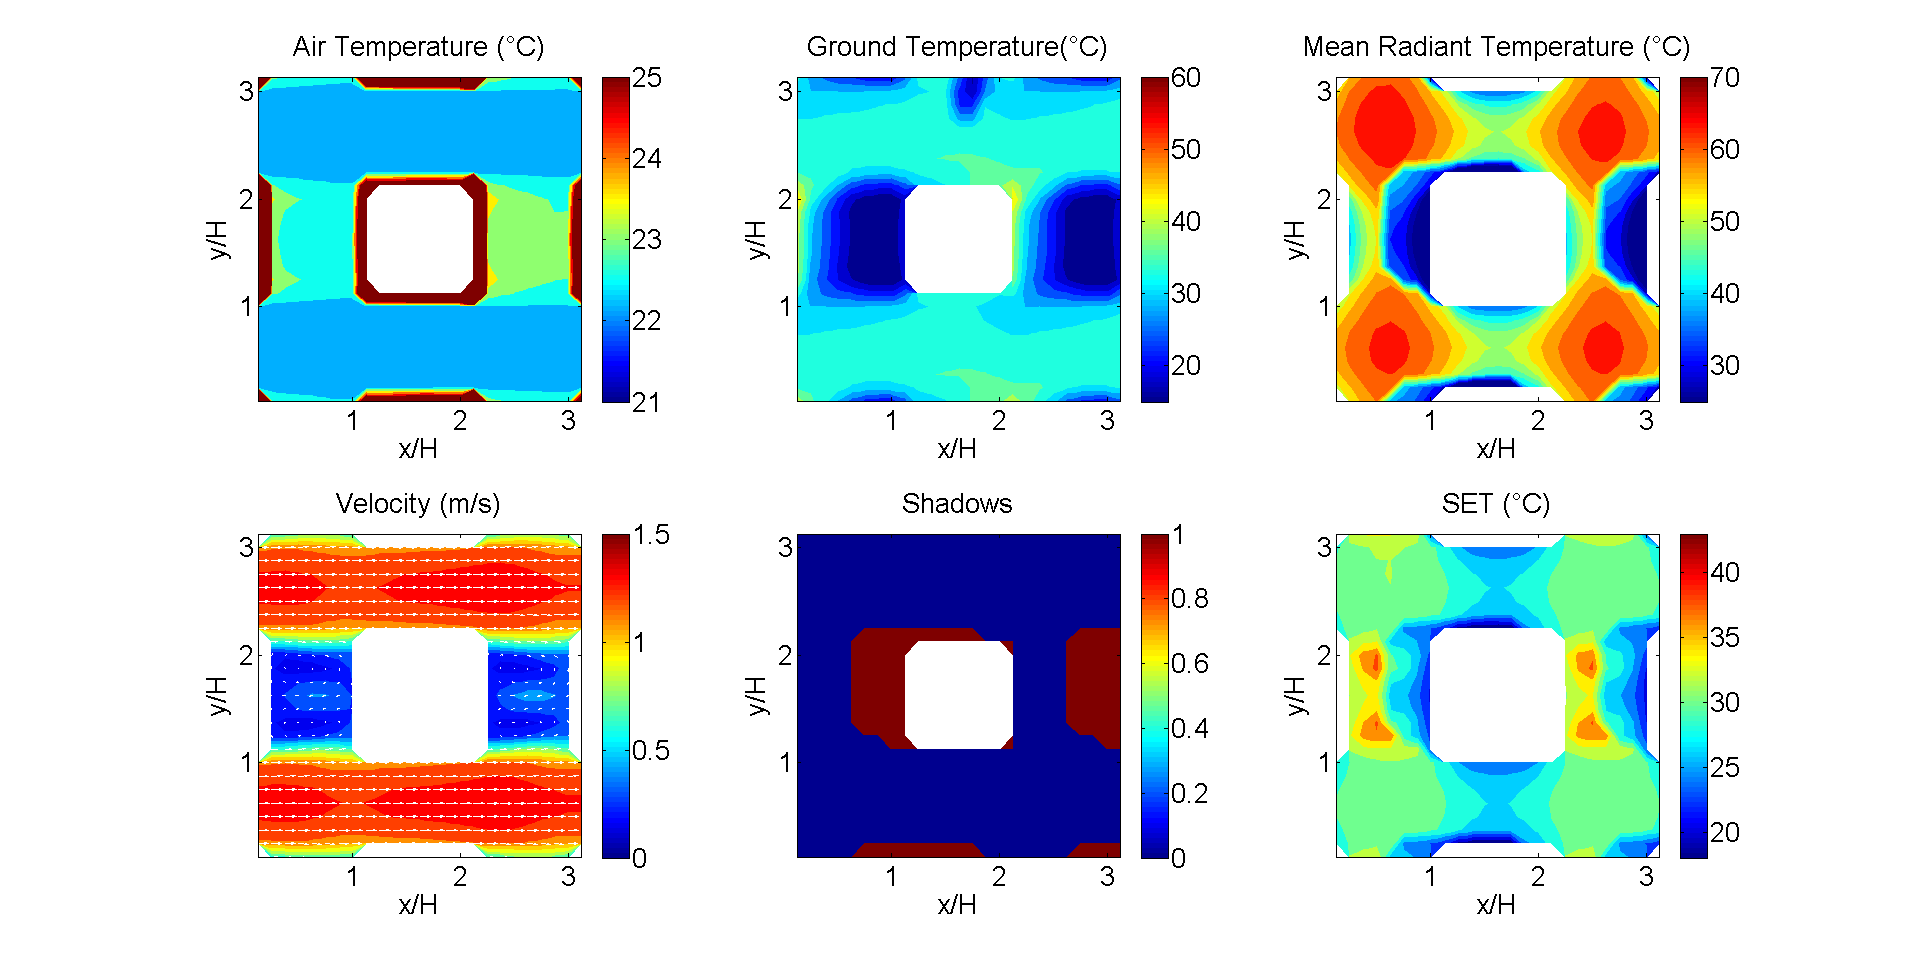
\includegraphics[width=\textwidth]{1000PST_flux.png}
\hskip 0.5in
\caption{Spatial distribution of different microclimate parameters affecting thermal comfort (SET) around a building at 1000PST.} 
\label{Fig.Parameters}
\end{figure}

The concurrent effects of micro-climate parameters in determining thermal comfort of pedestrians is evident. First, the results verify that despite the small variations in air temperature, SET is highly variable and unevenly distributed in a small urban area. Additionally, the vortex formation in the span-wise canyon in addition to the shading patterns have significant effects on the SET distribution at the pedestrian level. The vortex formation dramatically increases the SET in the span-wise canyon, while the shading enhanced the thermal comfort conditions, so that the same volume represents both best and worst position of pedestrian thermal comfort. Additionally, the effects of sky view factor and surface visibility are most apparent in the stream-wise canyon, where the thermal sensation is modified with respect to the pedestrians position. 

Spatial variation of thermal comfort is further demonstrated by evaluating the SET distribution along different paths in the street canyons. The two paths examined are shown in Fig. \ref{Fig.Paths}, followed by the variation of SET along these paths in Figs. \ref{Fig.LineSum} and \ref{Fig.LoopSum}. It can be seen that when the pedestrian is moving along the path through the stream-wise street, the thermal comfort experience has a small variability (maximum SET range of 3.9$^{\circ}$C at 1000 PST), whereas in the span-wise canyon the thermal sensation varies up to 14.6$^{\circ}$C. The comparison between streets parallel and perpendicular to the wind flow shows that the effect of wind patterns on SET are significant and should not be neglected, since vortex formation in the building canyons drastically increases SET values.  The effect of wind flow patterns can further be isolated by calculating SET in the isothermal simulation (Figs. \ref{Fig.LineSum} and \ref{Fig.LoopSum}), where uniform surface temperatures are considered and radiation effects are excluded.  As shown in the cross-canyon path, wind patterns create significant differences between span-wise and stream-wise canyons (up to 14 $\degree\,C$), and these differences are magnified when combined with the effects of shortwave radiation. In order to better evaluate the concurrent effects of wind and radiant exposure, a map of SET varied by $T_{mrt}$ and wind velocity is presented in Figure \ref{Fig.mapTV}. It can be seen that when the mean radiant temperature is high, small differences in wind speed result in large changes in thermal comfort. Conversely, when the wind speed is higher than 3-4 $m\,s^{-1}$, the difference in SET due to wind speed alteration is small. In other words, local wind velocity is a dominant factor when the radiant exposure is high (in sunlit places with high sky view factor or in the vicinity of high albedo surfaces) and when wind sheltering occurs in the street canyon. 

\begin{figure}[!h] \centering  
\graphicspath{ {image/} }
\begin{tabular}{cc}
 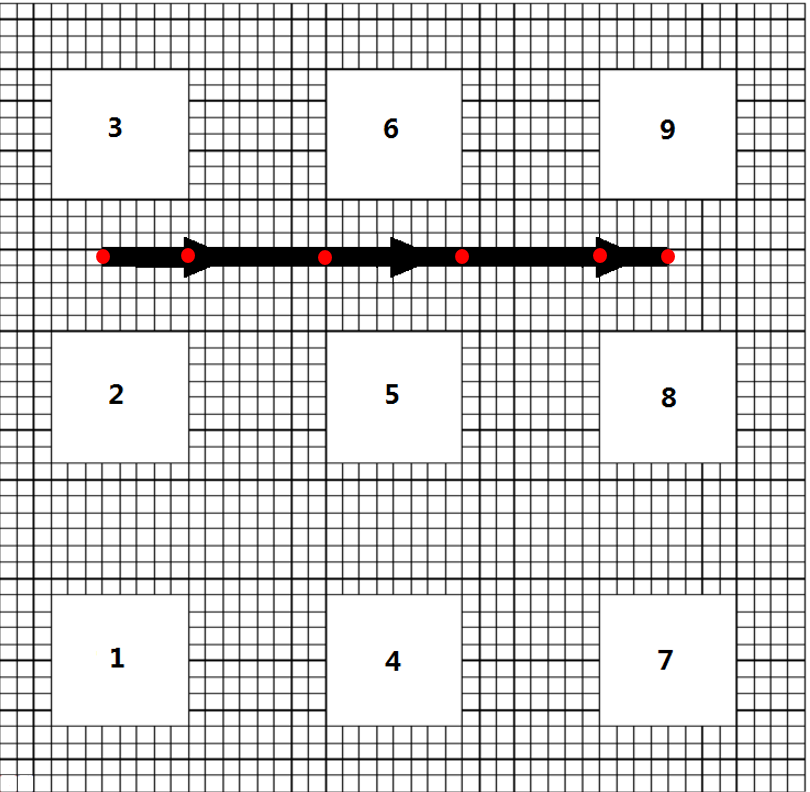
\includegraphics[width=.35\textwidth]{LineLocation.png}    &
 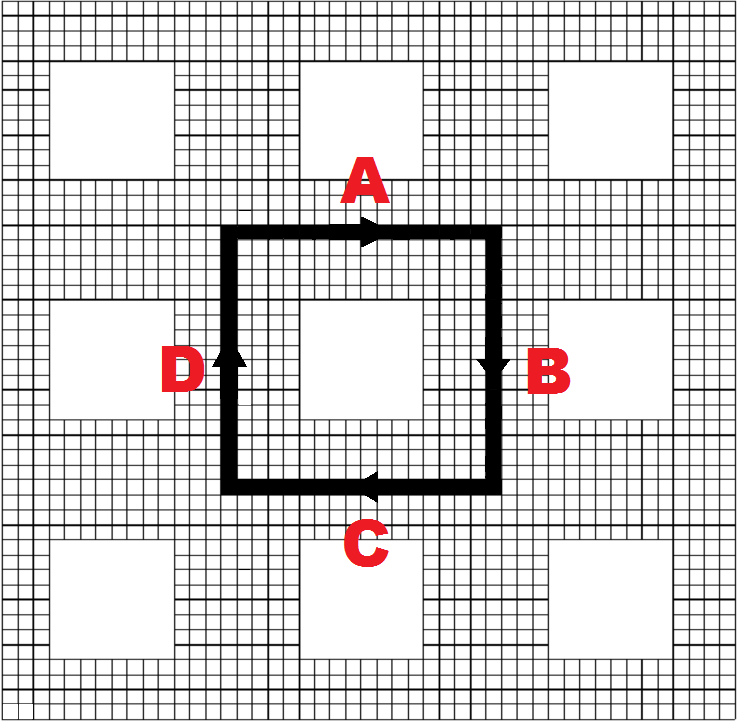
\includegraphics[width=.35\textwidth]{CircleLocation.png}   
\end{tabular}
\caption{Schematic of the pedestrian path in the urban area. The left figure represent the path through a stream-wise urban canyon, while the left graph is as if the pedestrian is walking around a building.} 
\label{Fig.Paths}
\end{figure}
   \begin{figure}[!h]
\graphicspath{ {image/} }
\centerline{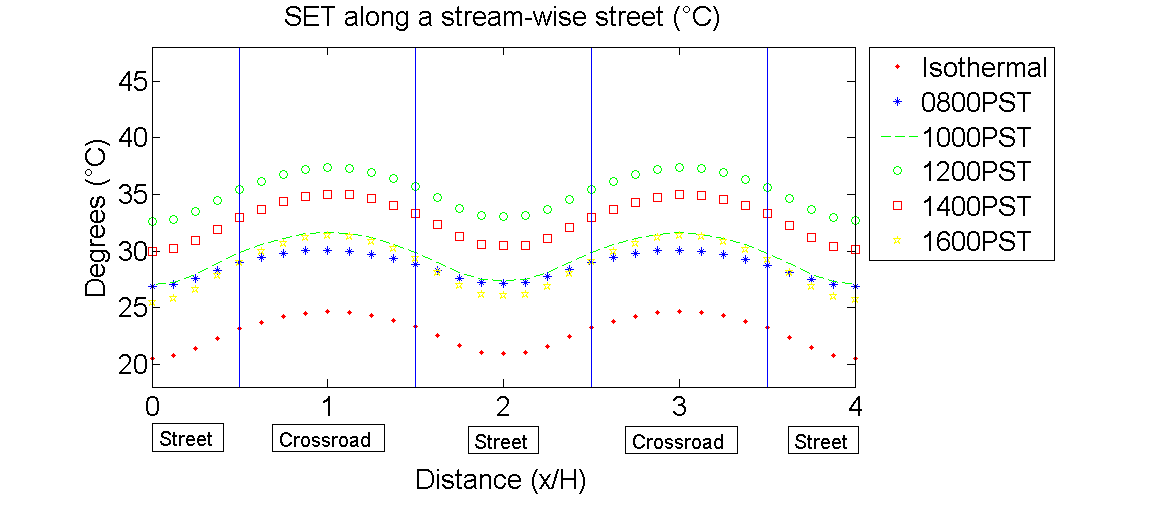
\includegraphics[width=0.95\textwidth]{line.png}}
\caption{SET distribution if the pedestrians are to follow a path along the stream-wise urban canyon, shown in Fig.  \ref{Fig.Paths}}
\label{Fig.LineSum}
\end{figure}
\begin{figure}[!h]
\graphicspath{ {image/} }
\centerline{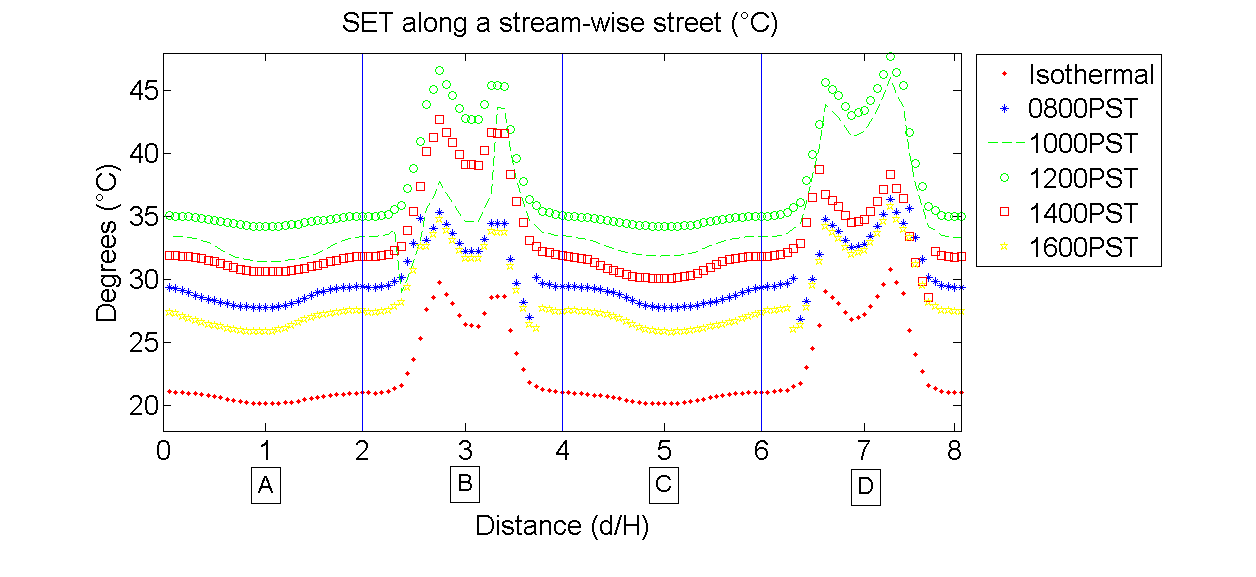
\includegraphics[width=0.95\textwidth]{loop.png}}
\caption{SET distribution if the pedestrians are to follow a path around a building, shown in Fig.  \ref{Fig.Paths}}
\label{Fig.LoopSum}
\end{figure}

\begin{figure}[!h]
\graphicspath{ {image/} }
\centerline{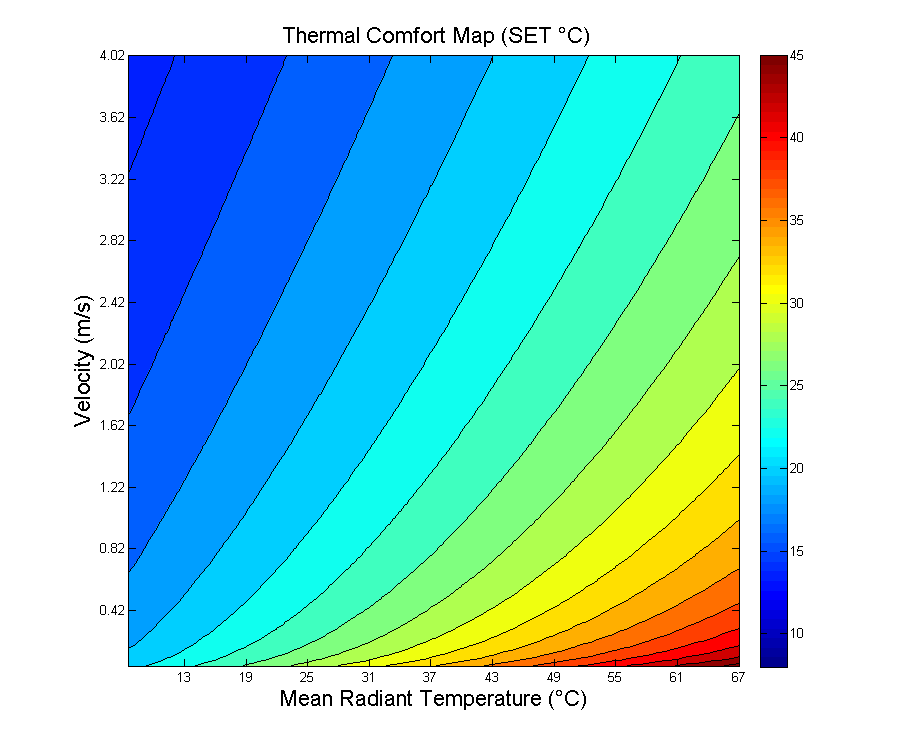
\includegraphics[width=10cm]{vel_mrt_map.png}}
\caption{Map of SET as a function of mean radiant temperature ($T_{mrt}$) and velocity.}
\label{Fig.mapTV}
\end{figure}

\subsection{Daily variation of thermal comfort: the effect of shortwave radiation and shading pattern}
The diurnal variation of thermal comfort is represented as the spatial distributions of SET values in Fig. \ref{fig:DiurnalDist}.  The SET distribution at the pedestrian level is calculated throughout the day from 0600 to 1800 PST in two hour intervals, and compared to the shade pattern demonstrated in the ground temperature distributions. A case with uniform surface temperature (isothermal) is simulated as the  point of reference. 

\begin{figure}[!h]
\centering
\begin{tabular}{cccll}
\cline{1-3}
\multicolumn{1}{|c|}{Isothermal Case} & \multicolumn{1}{c|}{0600 PST} & \multicolumn{1}{c|}{1000 PST} &  &  \\ \cline{1-3}
\multicolumn{1}{|c|}{\graphicspath{{image/}}
\raisebox{-\totalheight}{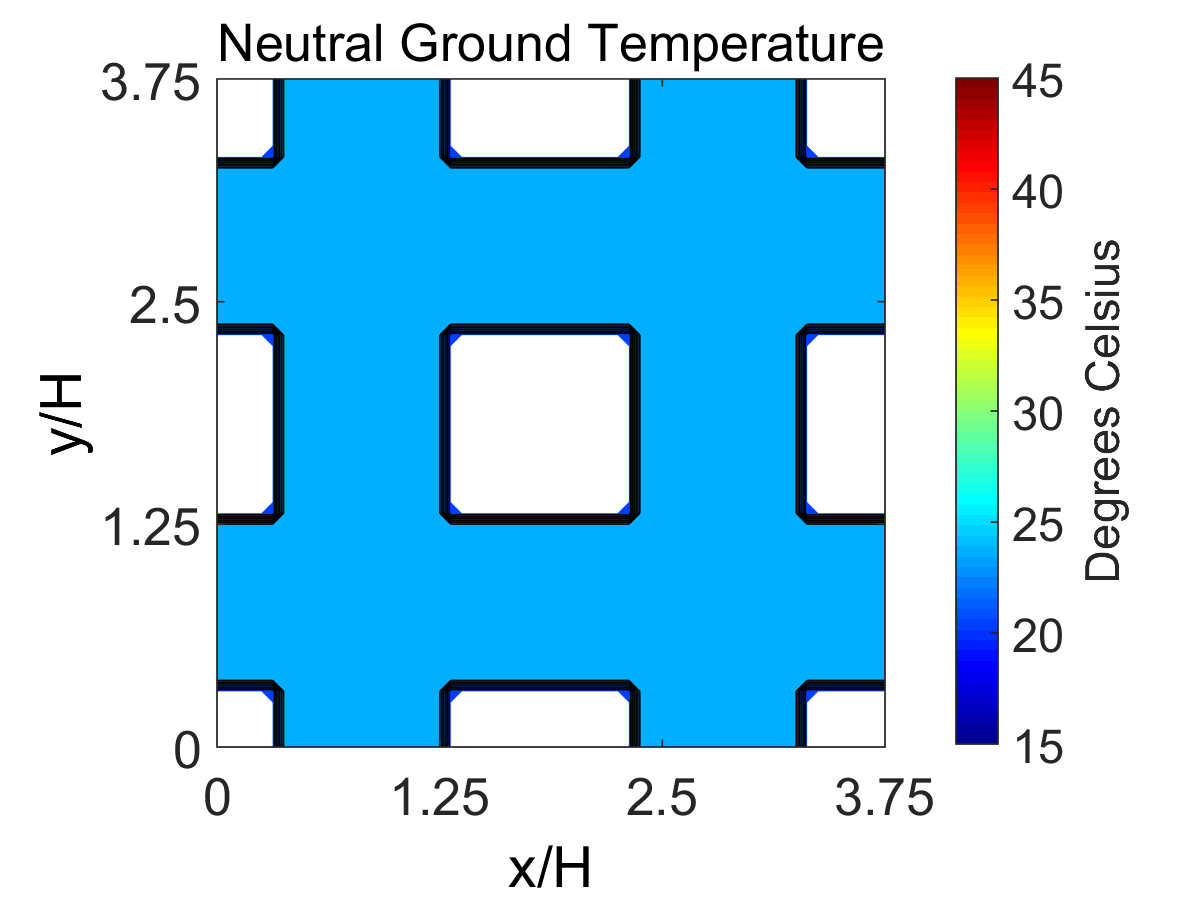
\includegraphics[width=0.3\textwidth]{GroundN.png}}} & 
\multicolumn{1}{c|}{\graphicspath{{image/}}\raisebox{-\totalheight}{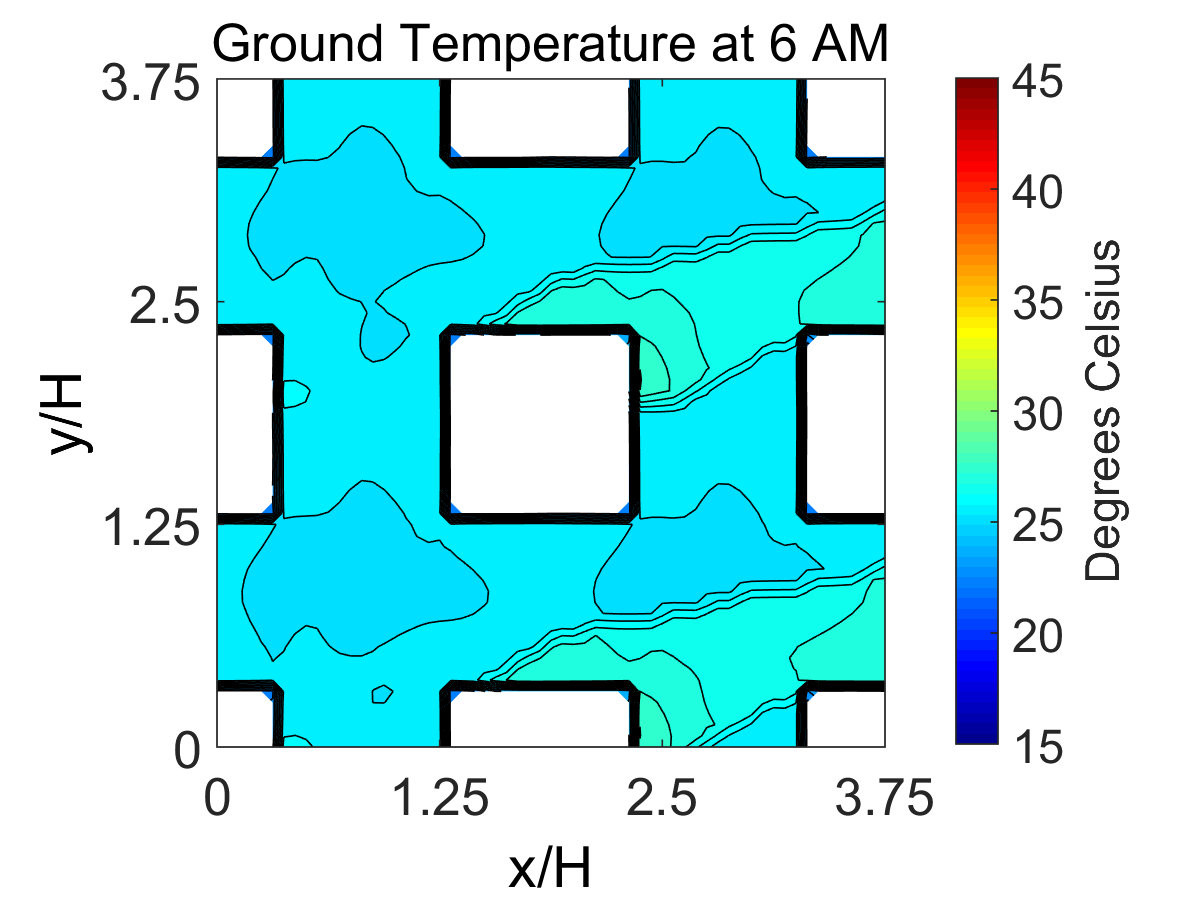
\includegraphics[width=0.3\textwidth]{Ground6AM.png}}} & 
\multicolumn{1}{c|}{\graphicspath{{image/}}\raisebox{-\totalheight}{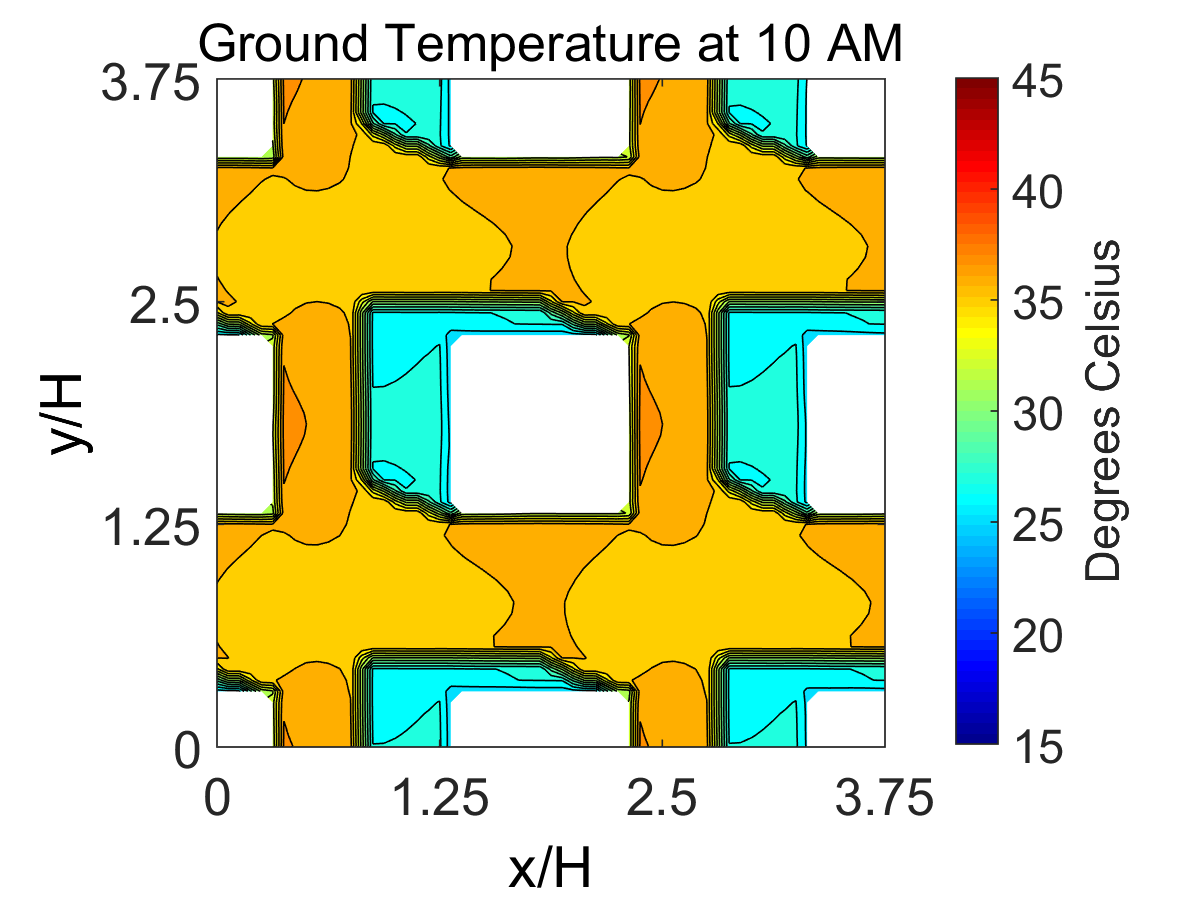
\includegraphics[width=0.3\textwidth]{Ground10AM.png}}}
&  &  \\ \cline{1-3}
\multicolumn{1}{|c|}{\graphicspath{{image/}}\raisebox{-\totalheight}{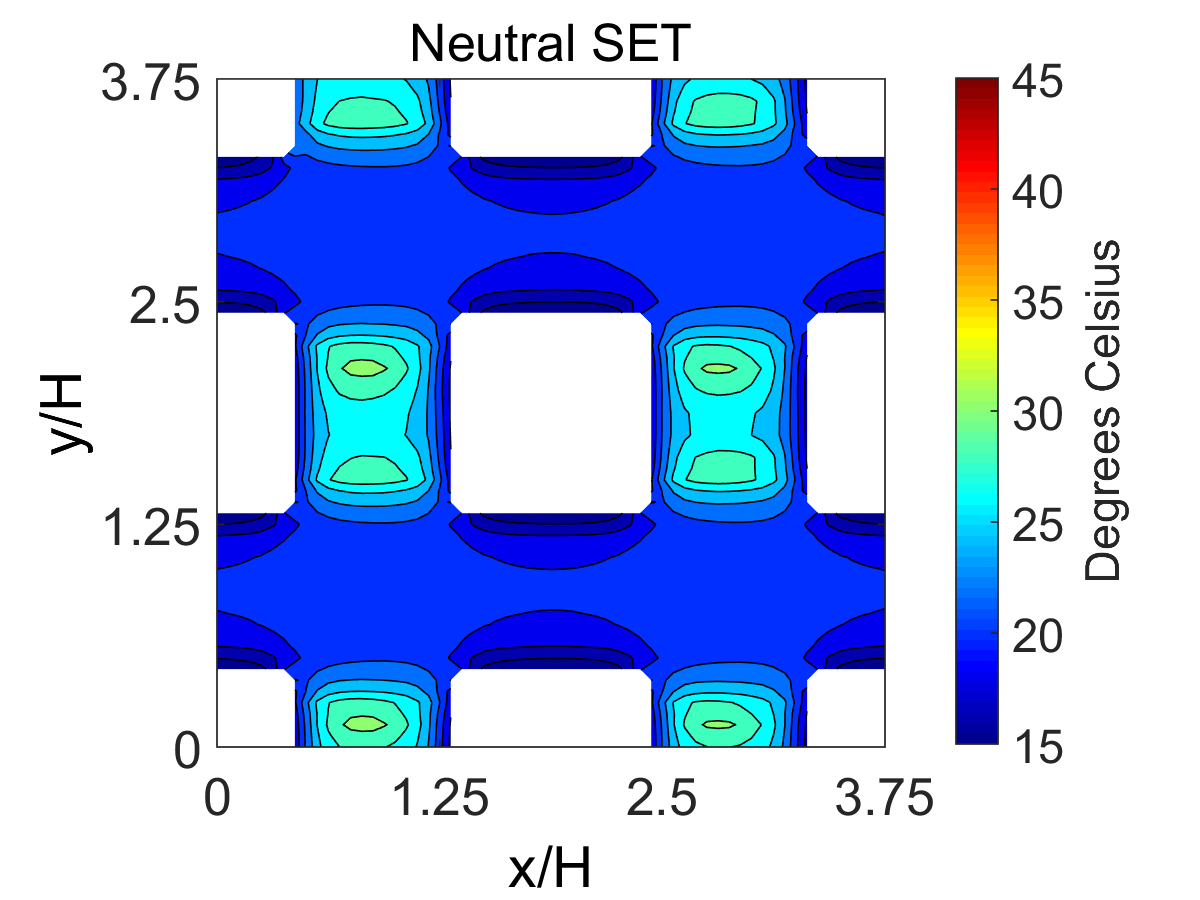
\includegraphics[width=0.3\textwidth]{SETNeutral.png}}} & 
\multicolumn{1}{c|}{\graphicspath{{image/}}\raisebox{-\totalheight}{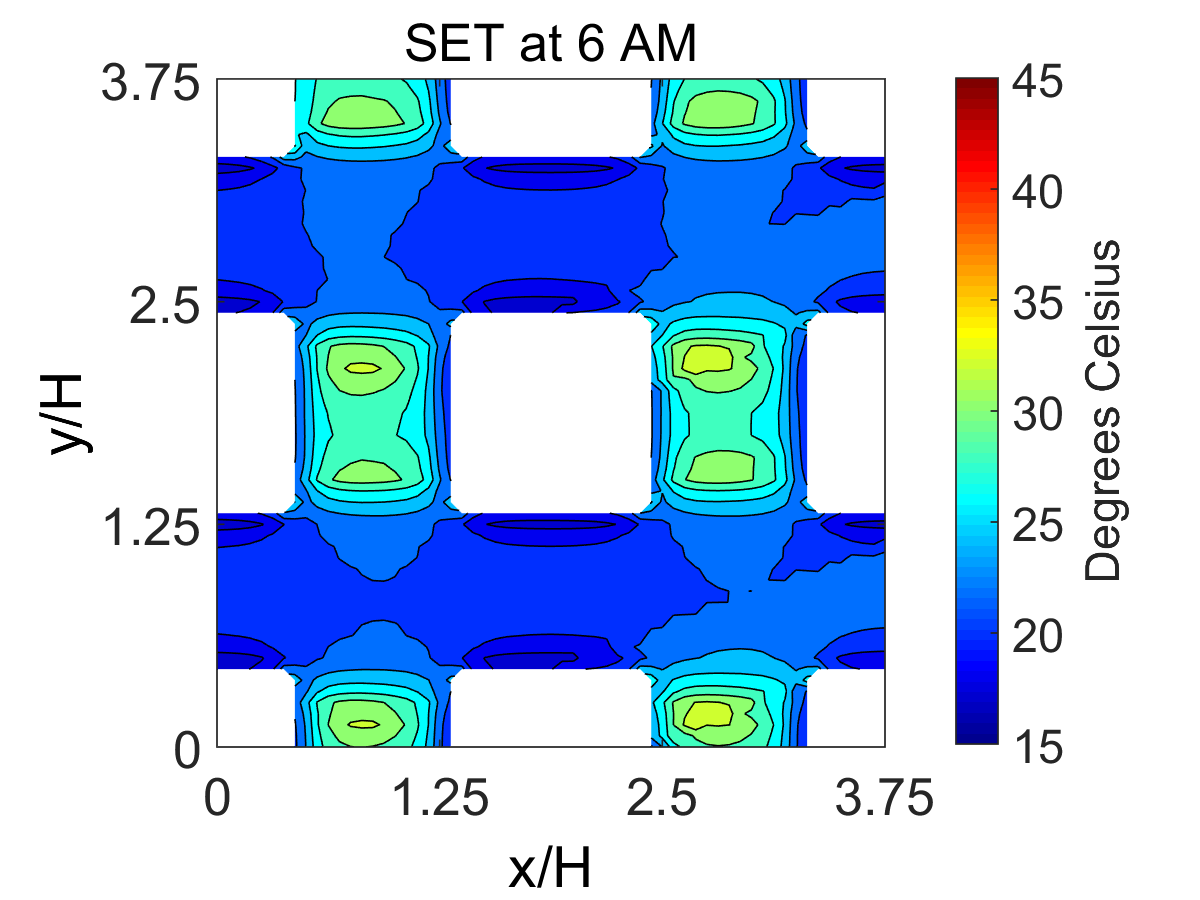
\includegraphics[width=0.3\textwidth]{SET6AM.png}}} & 
\multicolumn{1}{c|}{\graphicspath{{image/}}\raisebox{-\totalheight}{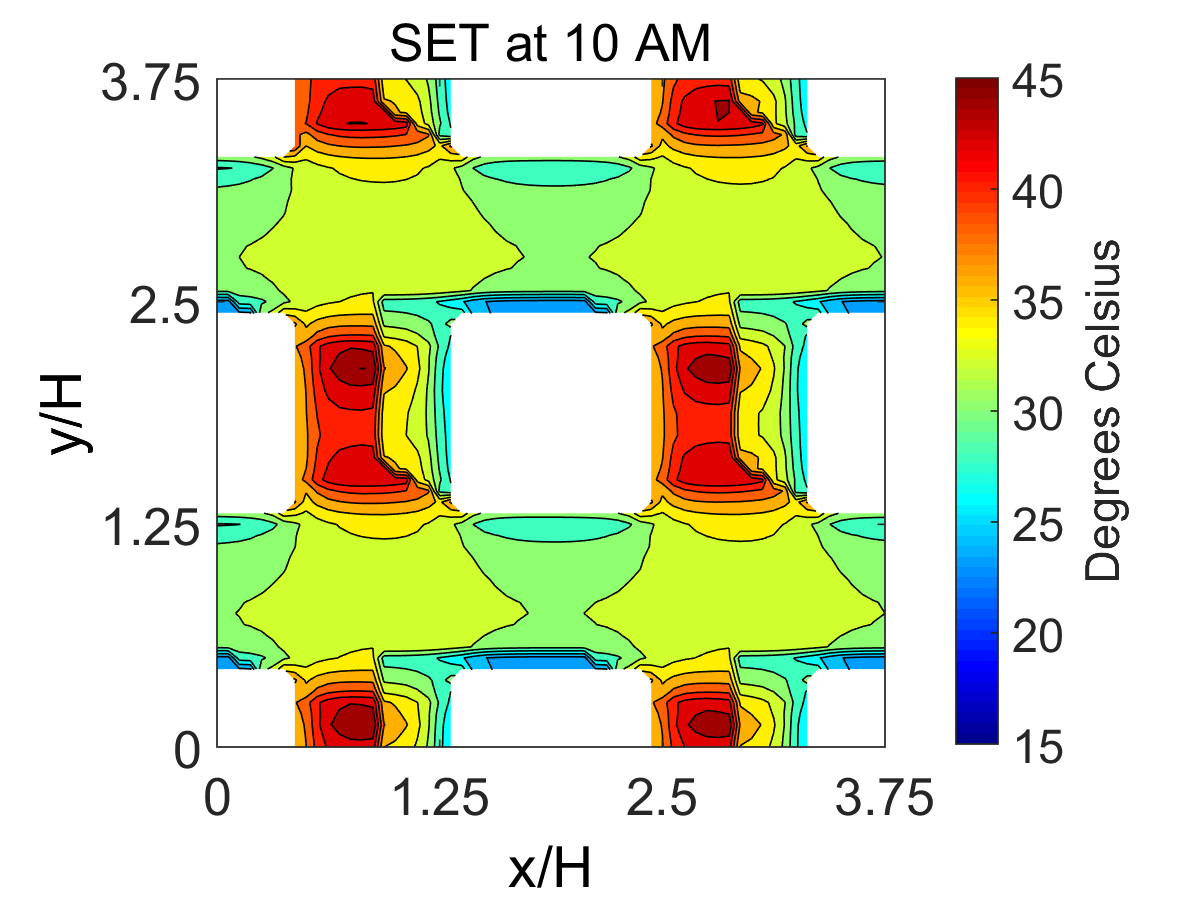
\includegraphics[width=0.3\textwidth]{SET10AM.png}}} &
&  \\ \cline{1-3}
                       &                       &                       &  &  \\ \cline{1-3}
\multicolumn{1}{|c|}{1200 PST} & \multicolumn{1}{c|}{1400 PST} & \multicolumn{1}{c|}{1800 PST} &  &  \\ \cline{1-3}
\multicolumn{1}{|c|}{\graphicspath{{image/}}\raisebox{-\totalheight}{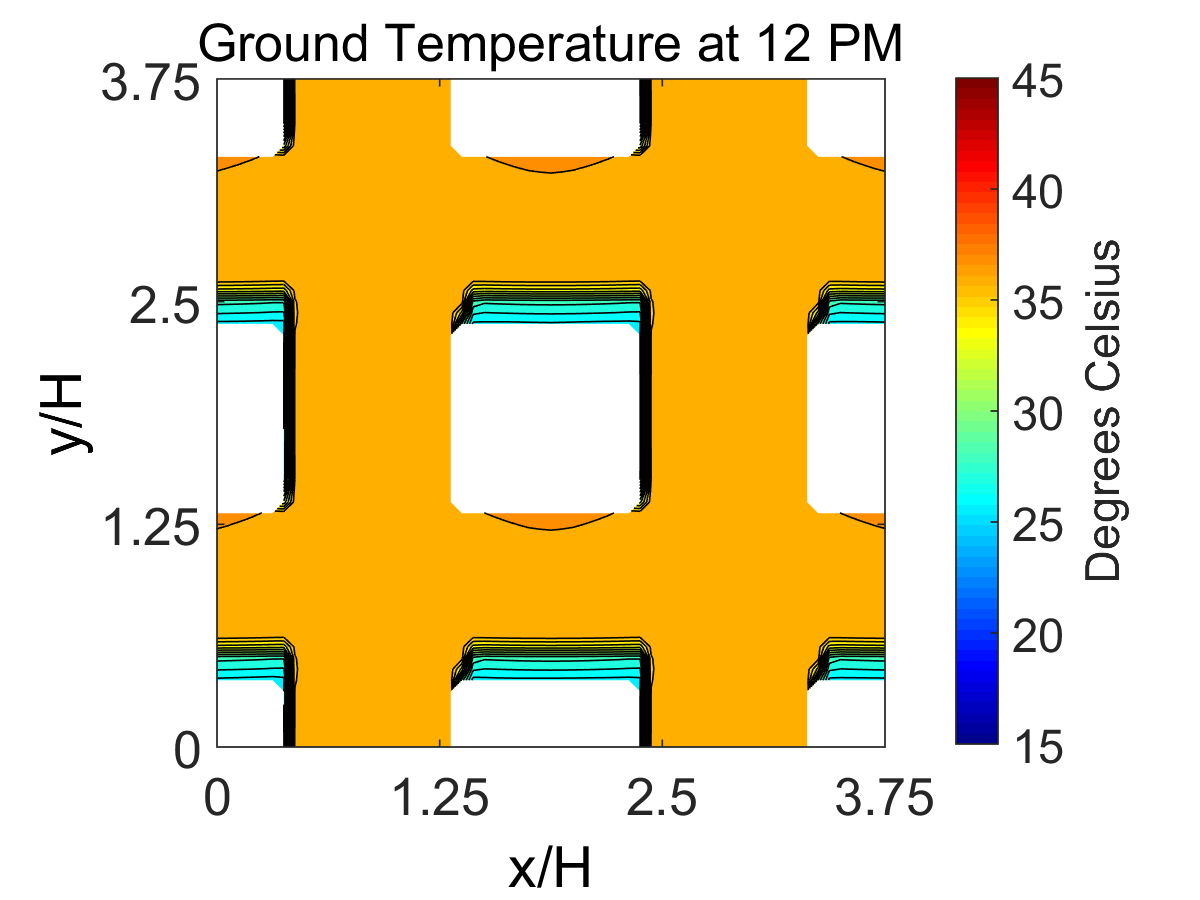
\includegraphics[width=0.3\textwidth]{Ground12PM.png}}} & 
\multicolumn{1}{c|}{\graphicspath{{image/}}\raisebox{-\totalheight}{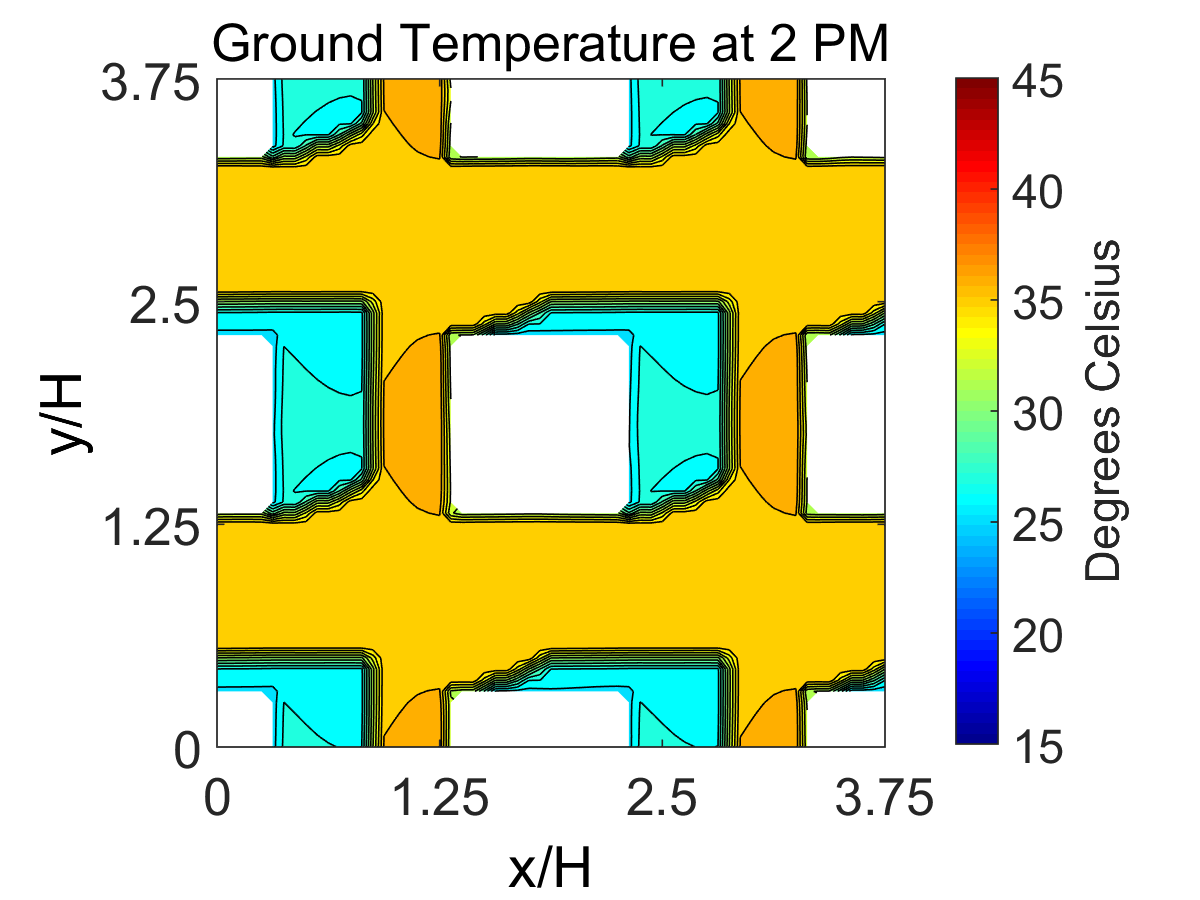
\includegraphics[width=0.3\textwidth]{Ground2PM.png}}} & 
\multicolumn{1}{c|}{\graphicspath{{image/}}\raisebox{-\totalheight}{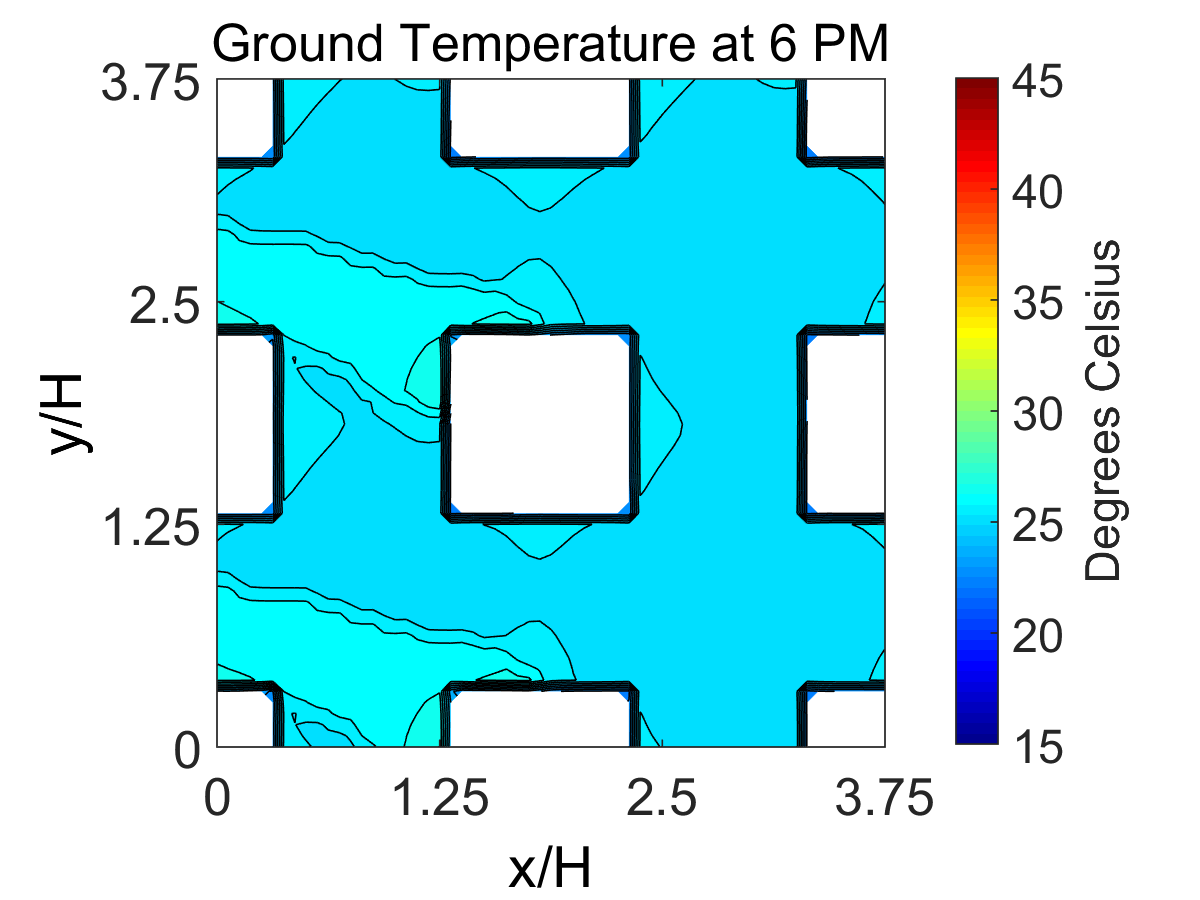
\includegraphics[width=0.3\textwidth]{Ground6PM.png}}} & &  \\ \cline{1-3}
\multicolumn{1}{|c|}{\graphicspath{{image/}}\raisebox{-\totalheight}{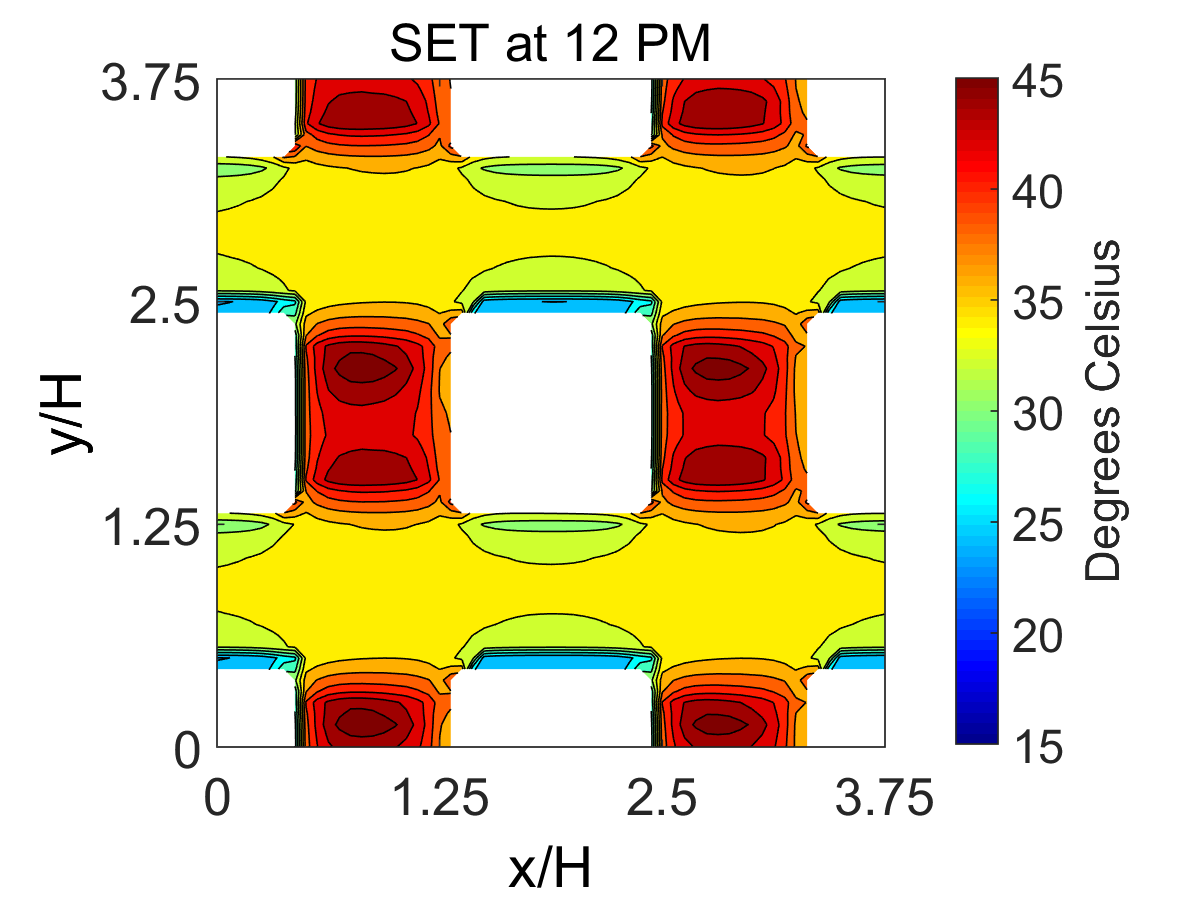
\includegraphics[width=0.3\textwidth]{SET12PM.png}}} & 
\multicolumn{1}{c|}{\graphicspath{{image/}}\raisebox{-\totalheight}{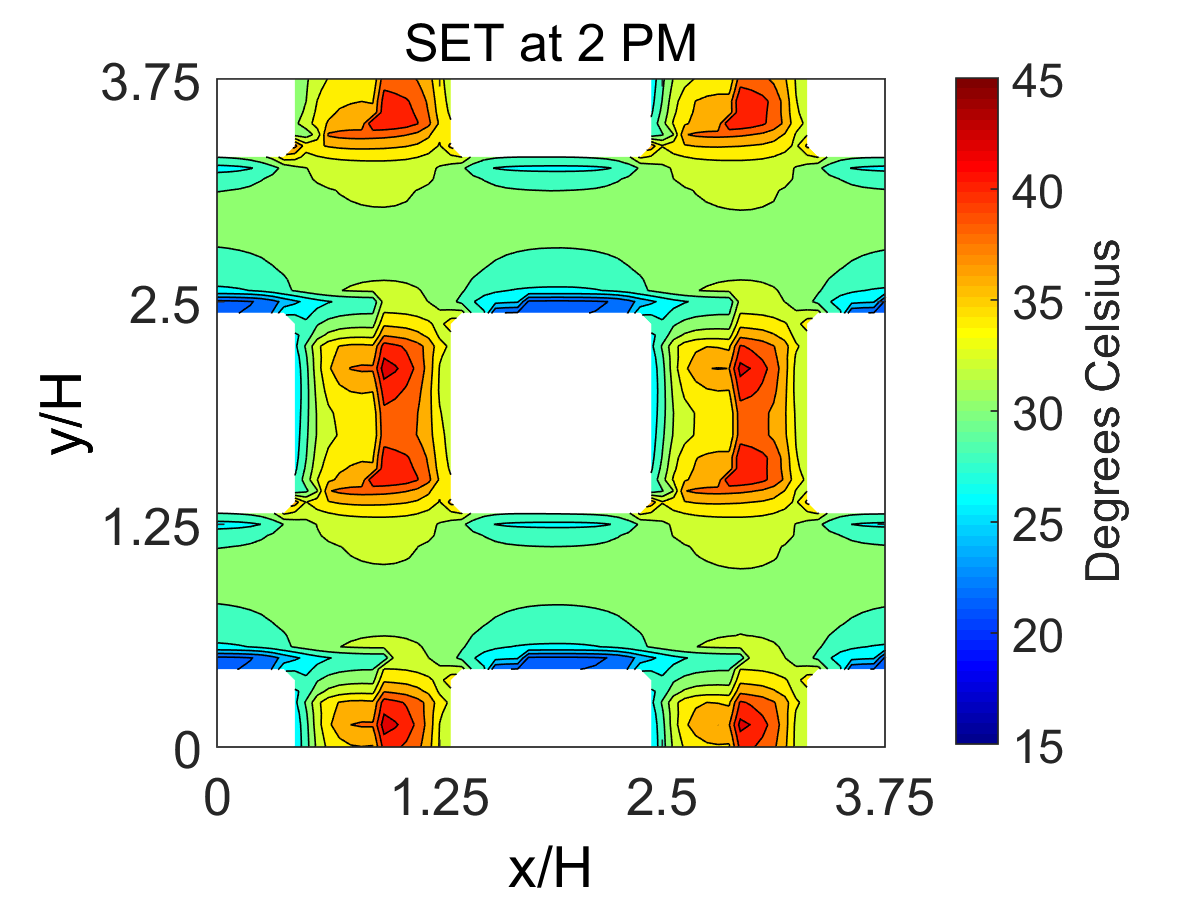
\includegraphics[width=0.3\textwidth]{SET2PM.png}}} & \multicolumn{1}{c|}{\graphicspath{{image/}}\raisebox{-\totalheight}{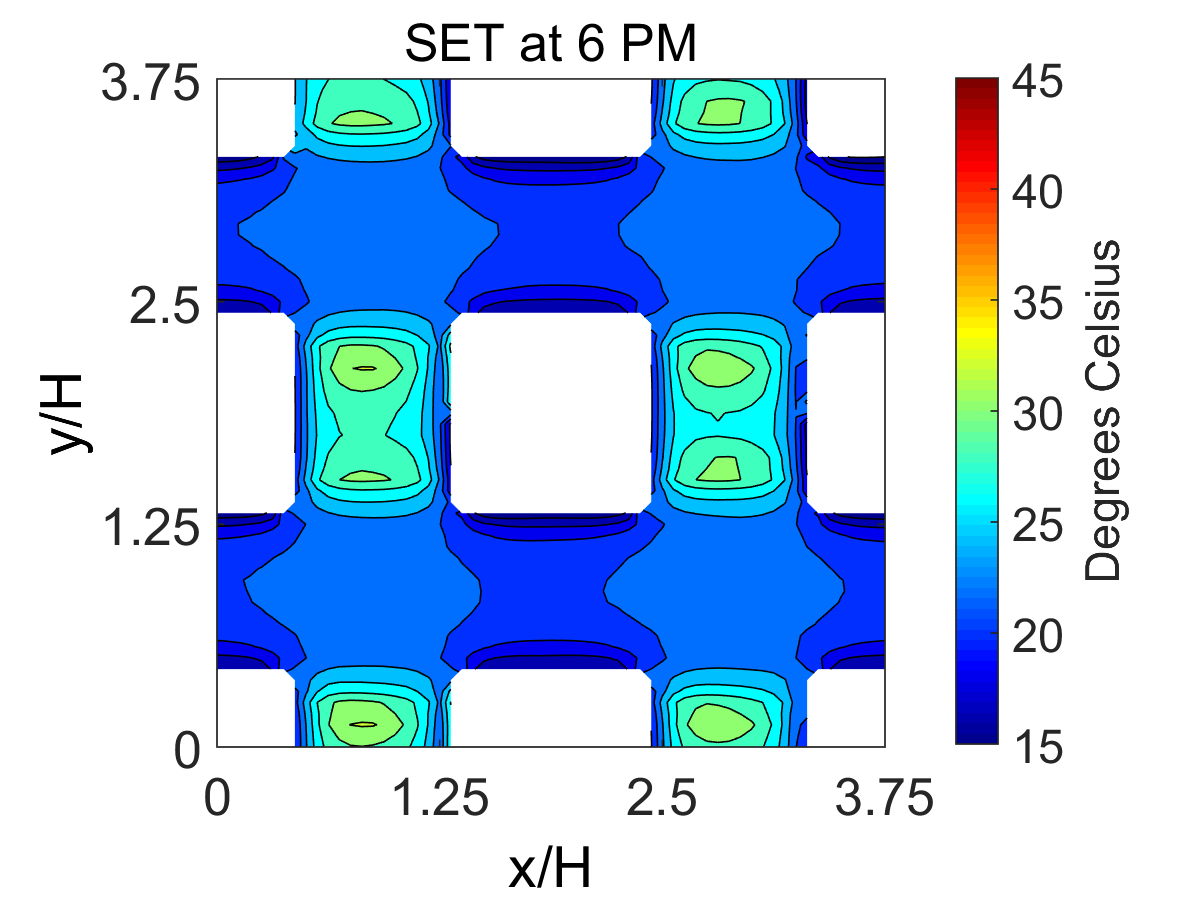
\includegraphics[width=0.3\textwidth]{SET6PM.png}}} &  &  \\ \cline{1-3}
\end{tabular}
\caption{Diurnal variation in ground temperature and SET distributions.}
\label{fig:DiurnalDist}
\end{figure}

Throughout the day, radiation exposure of the pedestrian changes with the solar angle when the shade pattern and shortwave radiation intensity are modified. Cases with approximately symmetric sun angles are compared (such as 1000 and 1400 PST) and it is seen that the shortwave radiation dominates the SET distribution more so than air temperature.   For instance, air temperature is the highest in the afternoon at 1400 PST, while the solar intensity as well as the SET value peak at noon (Fig. \ref{Fig.SolarIntensity}) where the position of sun minimizes the inter-building shadowing. Additionally, previous studies of unstable urban flow has shown the significance of heating orientation (windward vs. leeward heating) with respect to the wind direction, whereas thermal comfort seems to be insensitive to the heating orientation. 

The dominance of short-wave radiation on thermal comfort during daytime is demonstrated and the importance of shading in mitigating thermal stress is verified. Nonetheless, the effect of wind flow is evident in the span-wise canyon: a) in both cases of isothermal simulation and 1200 PST when the shading effects are excluded, the vortex formation has resulted in a dramatic increase in SET, and b) in the cases of 1000 and 1400 PST, even in the presence of shading, the thermal comfort is more adverse compared to the stream-wise canyon. These findings reveal the crucial importance of street ventilation on outdoor thermal comfort, and motivate more attention to the effect of urban design on street airflow.  
%talk more about location of sun

\subsection{Thermal comfort and wind direction}
When evaluating thermal comfort based on Eq. \ref{Eqa.SET}, wind direction is not an explicit variable in SET calculation. However,  wind direction modifies the flow field, and also changes the surface and air temperature distribution \citep{nazarian2014effects}. Accordingly, it is important to analyze the sensitivity of the SET distribution to the wind direction. Figure \ref{Fig.NWwind} shows the spatial distributions of flow and thermal fields, as well as SET at 1000 PST when the wind is blown from the northwest (45 degrees from the x-axis), while Fig. \ref{Fig.Swind} is obtained for wind direction from the south (90 degrees from the x-axis) at 1000 PST. These results indicate that wind direction substantially alters the SET distribution. When the wind direction is 45 degrees, the SET distribution pattern is markedly different, despite the identical ground temperature distribution. For instance, a local minimum value of SET is observed in the southern edge of the building where the wind speed is maximum, while the SET in both canyons is more uniform. Additionally, in the presence of strong wind sheltering and the absence of high wind velocity parallel to street canyon in the 45 degree case, thermal comfort is aggravated in all canyons. In the case of the 90 degrees wind direction, the SET distribution is  similar to the original 1000 PST distribution from Fig. \ref{fig:DiurnalDist}. For a better visual comparison, the coordinates are changed in this case and compared to the reference case of 0 degree wind with east-west axis \ref{Fig.SwindComp}. It can be seen that the average thermal comfort has increased 1$\degree C$ for the northbound wind direction, mainly due to the orientation of shading with respect to the wind direction. This analysis calls attention to the importance of wind direction on thermal comfort and more comprehensive analysis to be implemented in future. 
\begin{figure}[!h]
\graphicspath{ {image/} }
\centerline{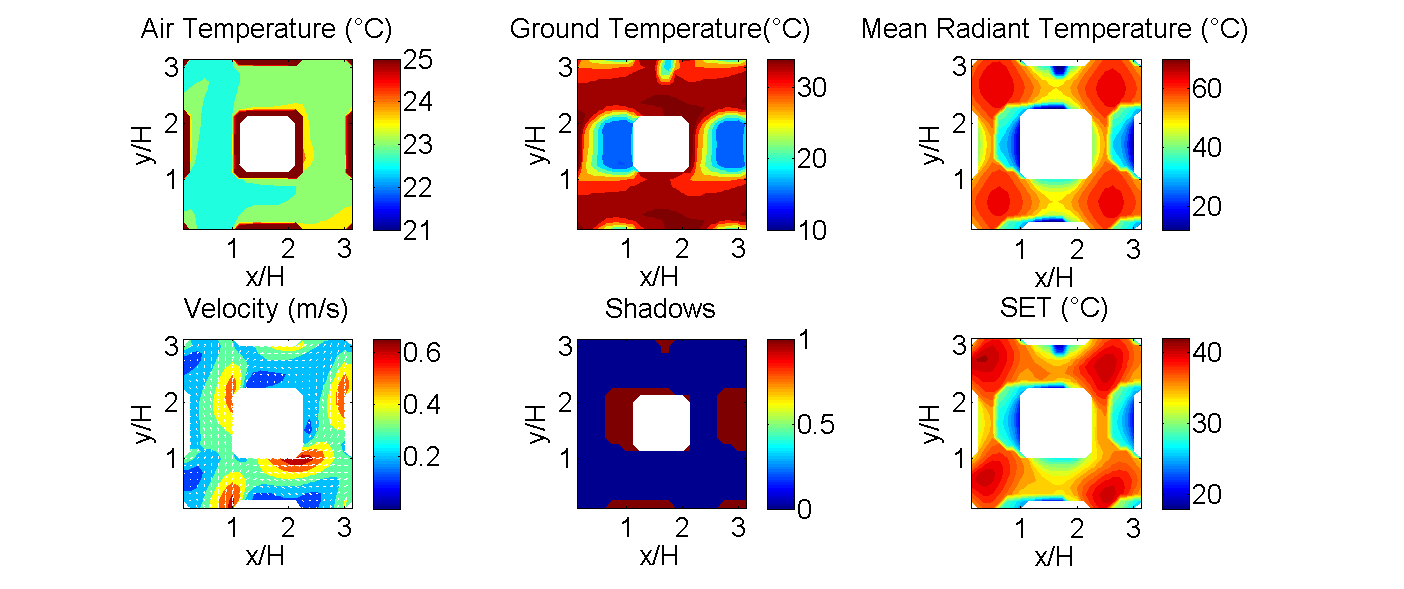
\includegraphics[width=\textwidth]{Theta45_10AM.png}}    
\caption{Spatial variation of SET at the pedestrian level for 1000 PST as wind direction is changed to 45 degree from the east-west axis.}    
\label{Fig.NWwind}
\end{figure}

\begin{figure}[!h]
\graphicspath{ {image/} }
\centerline{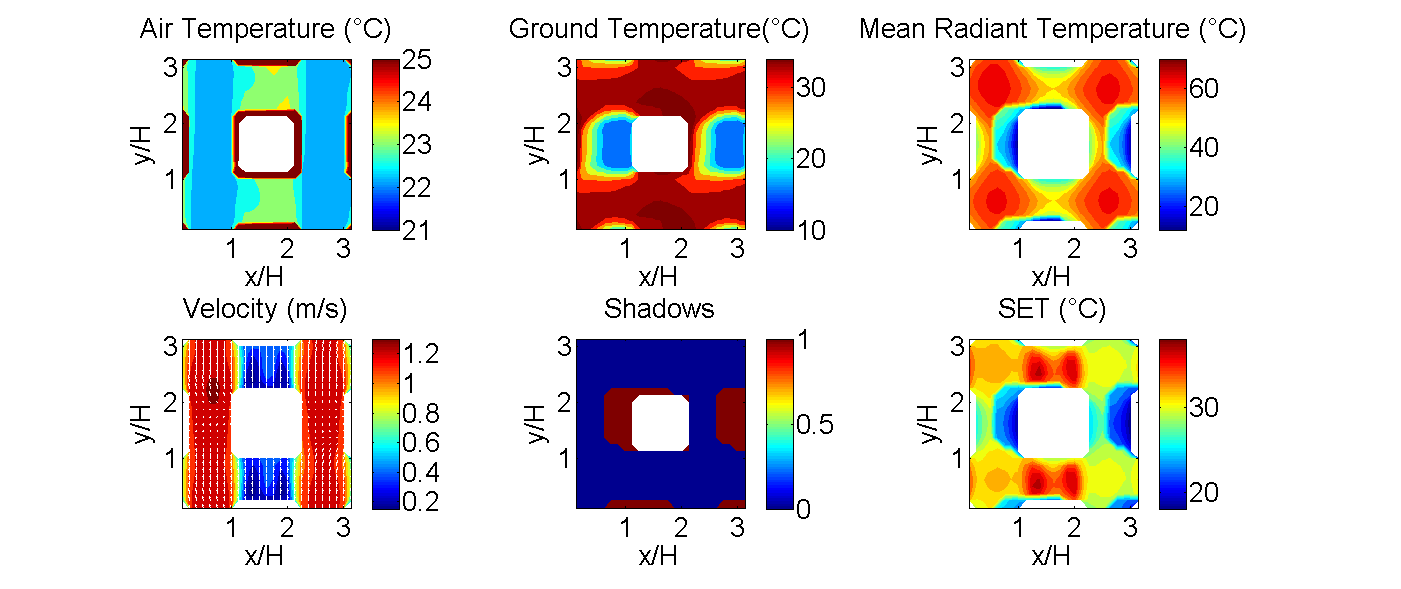
\includegraphics[width=\textwidth]{Theta90_10AM.png}}    
\caption{Spatial variation of SET at the pedestrian level for 1000 PST as wind direction is changed to 90 degree from the east-west axis.}  
\label{Fig.Swind}
\end{figure}

\begin{figure}[!h]
\graphicspath{ {image/} }
\centerline{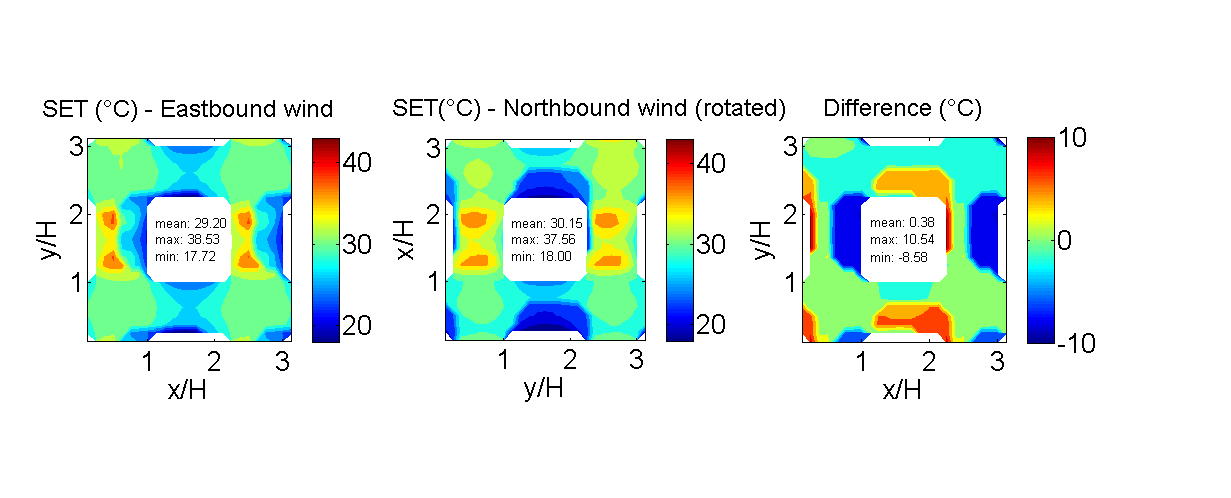
\includegraphics[trim= 0 1.8cm 2cm 1.7cm,clip=true, width=\textwidth]{compare_winds.png}}    
\caption{Spatial variation of SET at the pedestrian level for 1000 PST as wind direction is changed from 0 to 90 degrees from the east-west axis. The cases are compared by calculating the difference of SET in the right graph. }  
\label{Fig.SwindComp}
\end{figure}

\subsection{Thermal comfort and urban density}
Urban built-up density can be represented in the aspect ratio (AR) of the street canyons, i.e., the ratio of building height to street width (H/W). Street canyon aspect ratio affects wind flow, shade patterns and sky view factor. In our sensitivity study, the canyon ratio is modified by changing building spacing with constant building height. SET calculations of different aspect ratios are then conducted along the same line setup as in Figure \ref{Fig.Paths} at 1200 PST, so that the shortwave radiation and shading pattern remains the same at this path for all cases. 

\begin{figure}[!h]
\graphicspath{ {image/} }
\centerline{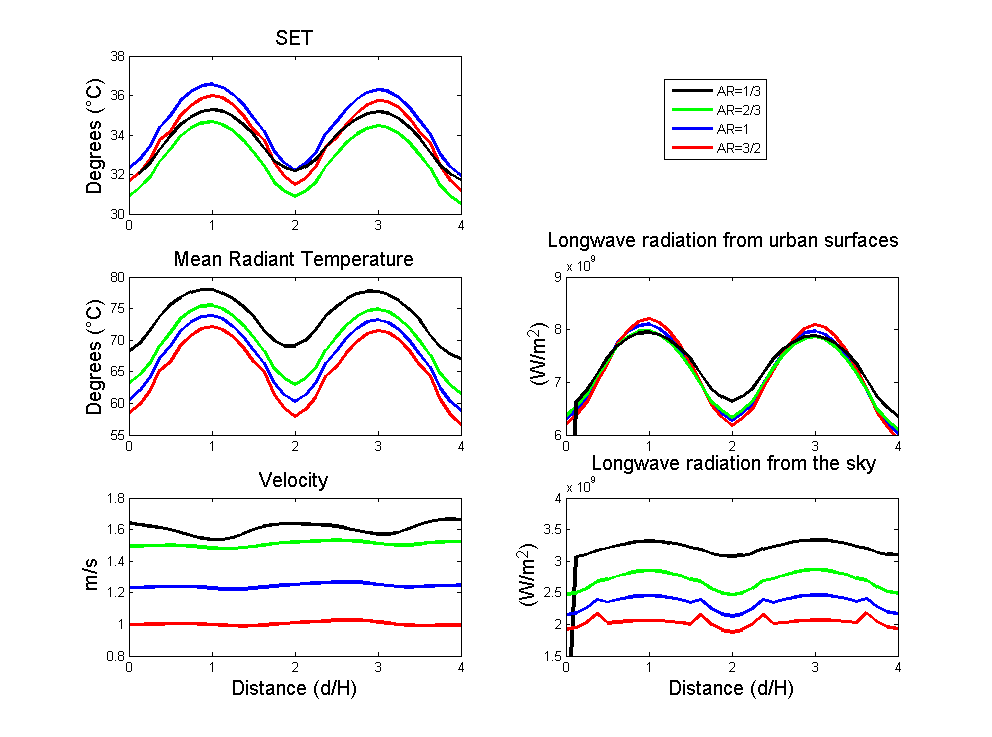
\includegraphics[width=\textwidth]{aspectratio_variables.png}}
\caption{SET distribution change with AR (AR is changed by higher building height therefore the location is referenced by width of buildings W)}
\label{Fig.AR}
\end{figure}

\begin{table}[!h]
\centering
\caption{Ranges in SET for varying aspect ratios}
\label{table:AR_range}
\begin{tabular}{llll}
  Aspect Ratio  & \textbf{min SET ($^{\circ}$C)} & \textbf{min SET ($^{\circ}$C)} & \textbf{Range ($^{\circ}$C)}\\ \hline
\multicolumn{1}{l|}{\textbf{1:3}} &     30.1     &     33.4      &   3.2        \\
\multicolumn{1}{l|}{\textbf{2:3}} &      30.5     &     34.7      &  4.2         \\
\multicolumn{1}{l|}{\textbf{1:1}} &      31.9     &     36.6      &   4.7       \\
\multicolumn{1}{l|}{\textbf{3:2}} &      31.2     &      36.0     &  4.8        
\end{tabular}
\end{table}

Figure \ref{Fig.AR} indicates that SET does not change monotonically with AR, due to the concurrent effects of various parameters. With increasing aspect ratio, sky view factor as well as visibility of urban surfaces decrease significantly, while wind sheltering increases. Therefore both mean radiant temperature and wind velocity decrease with counteracting effects on the SET. These concurrent effects are reflected in the SET calculations where increasing AR first enhanced thermal comfort by enhancing radiant exposure and further increased SET particularly in the crossroad.  However, it is possible that for a higher urban density, the effect of wind velocity as well as increased shading, temperature and energy waste into the canyon reverse the trend of thermal comfort. Therefore, the importance of further evaluating the design factors on thermal comfort is evident and can be used as a tool for adopting to current environmental concerns. 

%%%%%%%%%%%%%%%%%%%%%%%%%%%%%%%%%%%%%%%%%%%%%%%%%%%%%%%%%%%%%%%%%%%%%%%%%%%%%%%%%%%%%%%%%%%%%%%%%%%%%
\section{Conclusion and Future Perspectives}
\label{sec:conc}
Outdoor spaces are important to city design as they accommodate the urban dwellers and pedestrians in their outdoor activities. Accordingly, numerous studies has focused on improving outdoor spaces in terms of community, accessibility, and aesthetic aspects, with little or no attention given to the outdoor microclimate.  However, for a city to be “livable”, the outdoor experience should be of focus as much as the indoor characteristics. The thermal experience of pedestrians in outdoor spaces, i.e. outdoor thermal comfort, is an example of such concerns which calls for more in-depth analysis on the effect of urban design on microclimate. The current study is an example of achieving this objective.

In this study a methodology of evaluating thermal comfort in high spatial resolution is introduced. Standard Effective Temperature (SET) is taken as the metric of thermal comfort, and calculated in an idealized urban configuration using a comprehensive spatial model of mean radiant temperature incorporated with a detailed wind flow and thermal field simulations.  The following summarizes of the main findings:
\begin{enumerate}
    \item 	Spatial variability of thermal comfort: SET is shown to be highly variable based on the pedestrian location in the urban configuration, responding to the variation of flow field and radiant exposure in an urban configuration. 
    The spatial variability of sky view factor as well as visibility of urban surfaces also contribute to the variation of thermal comfort in urban environments, despite being often neglected. 
    \item 	Dominant factors of human comfort in outdoor environments: 
\begin{itemize}
\item \textbf{Mean radiant temperature} defines the radiant exposure of human and incorporates the radiation (longwave and shortwave) from the sun, urban surfaces, and the sky. 
It is expected and shown that $T_{mrt}$ dramatically changes the thermal sensation of humans, and among the 3 main factors mentioned here, shading is known to be the most dominant factors in $T_{mrt}$ calculation during the day. However, it is observed that the effect of SVF and visibility of surfaces is also significant and should not be neglected. For instance, when the aspect ratio is changed, for the same location and time of the day (meaning same direct and diffuse shortwave radiation), mean radiant temperature changes significantly. As these factors (sky view factor, visibility, and reflected radiation from the surfaces) are highly correlated with urban design, they can as well be employed for enhancing outdoor thermal comfort. 
\item Shading is known as the intuitive way of enhancing outdoor thermal comfort, while even in a shaded area, low \textbf{wind velocity} can dramatically worsen thermal comfort. In this study, we observe that SET can change up to 14 $\degree C$ due to the vortex formation in the building streets, even in the absence of direct solar radiation. The importance of wind speed is more apparent for higher mean radiant temperatures and in the presence of canyon vortex where the wind velocity can be near zero. 
\item 	During the day, the outdoor \textbf{air temperature} is dynamically modified with the radiation (shortwave and longwave), as well as conduction and convective heat transfer from the surfaces. However, in determining the variability of thermal comfort, it has shown to have a less significant effect.  On the other hand, during the nighttime when the UHI effect is the largest and solar heating is absent, it is expected that air temperature is a more direct factor in the spatial variability of thermal comfort.
\end{itemize}
\end{enumerate}

The presented work describes the framework of evaluating outdoor thermal comfort by combining detailed CFD simulations of urban flow with a more accurate model of $T_{mrt}$ calculation  Nonetheless, the proposed methodology is still under development and has yet to be expanded and evaluated. For a more comprehensive analysis, further research is required to answer the following questions and remarks:

\begin{enumerate}
\item The model of idealized urban configuration needs to be expanded to more realistic geometries representing urban areas, so that it can be used for future design decisions of already existing urban areas or new developments. A more detailed model is under-development by the authors which would also be more suitable for comparison with measurement and survey data.  
\item	Thermal comfort is a subjective perception of the thermal environment. Therefore, a complete evaluation and understanding of outdoor thermal comfort cannot be only achieved using merely numerical evaluation. There needs to be a two-way feedback between numerical results and field campaigns in order to evaluate the results. Accordingly, there is a need for data collection in urban areas, such as distribution of surface temperature, radiative properties, air flow distribution and mean radiant temperature in order evaluate the perceived thermal comfort, and correct the model for other possibly-determinant factors that should be included in the numerical analysis of thermal comfort. 
\item	Vegetation is an important factor in thermal comfort of urban dwellers, and yet one of the most complicated to be incorporated in the numerical analysis due to its multi-facet interaction with radiation, flow and evapotranspiration.  Therefore, further analysis needs to be done to consider vegetation in the future phases of this analysis.
\item	Further sensitivity analysis should be implemented that considers the effect of surface albedo, wider ranger of urban density as well as wind speed and direction on thermal comfort.  Additionally, the difference in thermal comfort metrics based on age, activity, and gender should be considered in order to have an inclusive analysis of human experience in outdoor environments. 
\end{enumerate}	


%%%%%%%%%%%%%%%%%%%%%%%%%%%%%%%%%%%%%%%%%%%%%%%%%%%%%%%%%%%%%%%%%%%%%%%%%%%%%%%%%%%%%%%%%%%%%%%%%%%%%

{\tiny \bibliography{reference}}
\bibliographystyle{abbrvnat}

\end{document}
